\documentclass[../thesis]{subfiles}
\graphicspath{{\subfix{../figures/}}}

\begin{document}
\chapter{Implementation}\label{ch:implementation}

\lettrine[lines=3]{\textcolor{Maroon}{R}}{elying} on the foundations of \SEE{} and the \glsentrylong{lsp} established in the previous chapter, we can now turn to the core part of this thesis:
The integration of \gls{lsp} into \SEE{}, with a special focus on how to build \glspl{city} using \gls{lsp}'s \glspl{capability}.
We will start by briefly going over some preliminary changes to both \SEE{} and the \gls{lsp} specification.
Then, we will spend the majority of this chapter specifying and explaining the algorithm which "converts" \gls{lsp} information into \glspl{city}, before looking into how additional \glspl{capability} can be integrated into \SEE{}'s \glspl{city} and \glspl{window}.
Finally, we will conduct a brief technical evaluation, with a more thorough user study following in the next chapter.

Before continuing with this chapter, I highly recommend watching the six-minute showcase video at \web{https://www.youtube.com/watch?v=yAzyv2\_q2ng}{2025-01-15}.
It goes over all important user-facing features implemented in this chapter and does a better job of presenting them than can be done in text alone.

\section{Preliminary Changes}
As promised in the preceding paragraph, we will first quickly list some preparations.

\subsection{Specification Cleanup}
While familiarizing myself with the \gls{lsp} specification, I noticed and fixed a few small issues along the way.
Most of these were of a formal nature (\eg, spelling, grammar, formatting, consistent usage of terms), some were fixing incorrect TypeScript syntax in the definition of \gls{lsp}'s data models.
The rest of the changes were related to the so-called snippet grammar.

In the context of \gls{lsp}, snippets are string templates that are inserted on certain completions (see \cref{subsec:unplanned}), with some designed parts being filled in by the programmer on insertion.
There are also parts that can be filled in by certain values (\eg, the file name), which can themselves be transformed using regular expressions.\footnote{
	I am skipping over some additional features and details here because this is not that relevant a \gls{capability} for us---to get the full picture, see \web{https://microsoft.github.io/language-server-protocol/specifications/lsp/3.18/specification/\#snippet\_syntax}{2024-10-10}.
}
The complexity of the combinations of all these features increase the possibility of misunderstandings, which is why the snippet's grammar has been formally specified in \gls{ebnf}.
However, as it was written down in the specification, the grammar had a few problems that I have fixed.
Three notable examples are:
\begin{itemize}
	\item Some alternatives were incorrectly grouped, contradicting the explanatory text above them.
	      Also, the rules on how and when control characters had to be escaped were inconsistent with the surrounding text.\footnote{
		      This has lead to confusion in some projects making use of snippets.
		      See, for example, \web{https://github.com/neovim/neovim/issues/30495}{2024-10-10}.
	      }
	\item The grammar contained some string transformations that were unexplained in the text.
	      Since the \gls{lsp} specification is based on \gls{vscode}, I added explanations to the text based on what these transformations did in \gls{vscode}'s source code.
	\item Finally, there were ambiguities present in the grammar that led to \textsf{FIRST}/\textsf{FOLLOW} conflicts.
	      I have rewritten the grammar to eliminate these, and it should now be $LL(1)$-parseable~\cite[222--224]{aho2007}.

\end{itemize}


I have submitted these fixes as a pull request\footnote{\web{https://github.com/microsoft/language-server-protocol/pull/1886}{2024-10-10}}.
After addressing the resulting code review, it has been merged, and the changes will be incorporated in the upcoming 3.18 release of the specification.

\subsection{Preparing SEE}
There was not much I had to do in terms of getting \SEE{} ready, so this section will be short:
\begin{itemize}
	\item I have integrated the OmniSharp \gls{lsp} C\# library~\cite{csharplanguageserverprotocol2023} into \SEE{}, which we will leverage in the subsequent sections so that we can use \gls{lsp} without needing to worry about \gls{jrpc} encoding, data models, and so on.
	\item \Glspl{window} have previously been made editable by \textcite{moritz} in his bachelor's thesis, also enabling collaborative editing over the internet.
	      I unfortunately had to remove these changes because they did not work anymore in the current version of \SEE{}, and additionally caused a lot of complexity overhead in the \gls{window} implementation that would have made the \gls{lsp} integration much harder.
	\item Finally, the attribute space $\mathcal{A}$ in \SEE{} did not allow for \glspl{range} of the form \gls{lsp} needs, so I had to replace the existing attributes (which track the line and column, but not a full range) with a proper set of \gls{range} attributes.
	      In \cref{subsec:graph}, we have introduced this as a single \tt{Source.Range} attribute, but in reality, there are four \gls{range} attributes---one per member of the decomposed form.
	      We will ignore this reality for the rest of this thesis and act like the \gls{range} is a single attribute, that is, for all project graphs with nodes $V$ and attributes $a$, it holds that $\{a(v, \tt{Source.Range}) \mid v \in V \land (v, \tt{Source.Range}) \in \mathrm{dom}(a) \} \subseteq \mathcal{R}$.
\end{itemize}

All of these changes have been made across two pull requests to \SEE{}.\footnote{
	\url{https://github.com/uni-bremen-agst/SEE/pull/687} and \web{https://github.com/uni-bremen-agst/SEE/pull/715}{2024-10-11}.
}

\section{Generating Code Cities using LSP}\label{sec:generate}
In this section, we will examine the centerpiece of this thesis:
The algorithm with which \glspl{city} can be generated using the \glsentrylong{lsp}.
While going over how the algorithm works, we will investigate \glspl{intervaltree} and how they relate to the algorithm, before finally taking a look at what the import process looks like in practice in \SEE{}.

\subsection{Algorithm}

We will examine the algorithm in a generalized and programming language independent form here.
In this form, the algorithm takes as input a set of source code documents, as well as a family of \gls{lsp} functions belonging to a specific instantiation of a \gls{ls}.
These functions will be used to analyze the documents and extract the required information from them.
The output of the algorithm, is a graph representing the given software project.
\fxnote{Improve coloring of inner boxes and reduce height of boxes.}

\begin{figure}
	\begin{center}
		\includegraphics{tikz/algorithm.tikz}
	\end{center}
	\caption{A high-level overview of the basic steps of the algorithm.\\
		"\textcolor{red}{\textbf{!}}" represent diagnostics, while "\textcolor{red!30}{\textbf{!}}" represent aggregated diagnostics.
	}\label{fig:alg_overview}
\end{figure}

\paragraph{Overview}
Before diving into the specifics of \emph{how} the algorithm works, it may help to take a look at the diagram in \cref{fig:alg_overview}, which gives us a high-level overview of \emph{what} it does.
To summarize, the steps can be broken down into three major parts:
\begin{enumerate}[label=\bfseries\Roman*]
	\item \textbf{Node Synthesis:} Here, we create the graph's nodes and combine them together into a hierarchy.
	      \begin{enumerate}[label=\arabic*.]
		      \item We recreate the parts of the filesystem hierarchy that are relevant to the given documents (\ie, directories the documents are contained in and their relation to each other).
		      \item For each code symbol within that document, a node will be created as a child to the document.
		            Any symbols contained within that symbol are recursively added in the same manner as a child to their parent nodes.
		      \item Finally, we will pull diagnostics for the document\footnote{
			            In the actual algorithm, we cannot rely on pulling diagnostics alone, since only few \glspl{ls} support this.
			            Instead, we will collect pushed diagnostics in the background and handle them all at once at the very end.
		            } and attach their counts to the nodes they correspond to.
	      \end{enumerate}
	\item \textbf{Edge Synthesis:} Here, we connect the nodes by creating edges between them.
	      To do this, we go over each node, using \gls{lsp} functions to check for definition locations, references, and so on, and then determine which of our existing nodes best corresponds to that location.
	      This turns out to be the most difficult and complex part of the algorithm to implement efficiently, as we will later see.
	\item \textbf{Aggregation:} Finally, we want to aggregate \gls{loc} and diagnostic count metrics upwards in the hierarchy.
	      This way, we can, for example, see how many diagnostics are contained as a whole in a class, or even a directory.
\end{enumerate}

\paragraph{Specification}
Now that we know what it is the algorithm does, we can take a look at its detailed specification.
The specification is given in \cref{alg:generate} and follows a few special formatting rules that I will briefly list here:
\begin{itemize}
	\item Text in \textsc{Small Caps} refers to functions.
	      Those starting with \textsc{Lsp} specifically refer to functions provisioned by the \gls{ls}.
	\item Sentences in \textit{\textcolor{gray}{gray italics}} are comments.
	\item \textbf{Bold} text represents keywords.
	\item A normal font represents strings (\ie, text that represents itself).
	\item Finally, parts in a \texttt{typewriter font} serve two purposes:
	      They represent attribute keys ($\in \mathcal{A}_K$) as well as properties of \gls{lsp}-returned objects, the latter of which are prefixed by a dot.
\end{itemize}

\Cpageref{alg:generate} contains the main algorithm.
We can map \cref{fig:alg_overview} onto it as follows:
\Crefrange{alg:generate:begin}{alg:generate:end1} contain part I (node synthesis),
\crefrange{alg:generate:end1}{alg:generate:end2} contain part II (edge synthesis),
and finally, \crefrange{alg:generate:end2}{alg:generate:end3} contain part III (aggregation) as well as handling of pushed diagnostics.

The following \cpagerefrange{alg:generate:funcstart}{alg:generate:funcend} contain the functions referenced in the main algorithm.
Here, we represent the "types" of each parameter by specifying the function domain, that is, by noting the sets each parameter must be in.
Most of these sets are already defined in \cref{ch:concepts} or the algorithm itself, but two exceptions to this are the set of \gls{lsp} code symbols~$\mathcal{S}$ and the set of \gls{lsp} diagnostics~$\mathcal{D}$ (not to be confused with the set of input documents~$D$).

\tikzexternaldisable

\begin{algorithm}
	\small

	\floatname{algorithm}{Algorithm}
	\caption{How \gls{city} graphs can be generated from \gls{lsp} information.}\label{alg:generate}
	\begin{algorithmic}[1]
		\Require  {Family of \textsc{Lsp} functions provided by the \gls{ls}}, {set of documents $D$}
		\Ensure {Graph $G$ representing the underlying software project}
		\Statex
		\State $V, E, a, s, t, \ell, C \gets \varnothing$ \Comment{Initialize empty graph components.}
		\label{alg:generate:begin}
		\ForAll{$d \in D$}
		\State \Call{LspOpenDocument}{$d$} \Comment{Document needs to be opened for all capabilities to work.}
		\State $v_d \gets$ \Call{AddDocumentNode}{$d$} \Comment{Each document becomes a node\dots}
		\ForAll{$x \in \textsc{LspDocumentSymbols}(d)$}
		\State \Call{MakeChild}{\Call{AddSymbolNode}{$x$}, $v_d$} \Comment{\dots with its symbols as children.}
		\EndFor
		\If{\Call{LspLanguageServerSupportsPullDiagnostics}{\null}}
		\State \Call{HandleDiagnostics}{\Call{LspPullDocumentDiagnostics}{$d$}}
		\Else
		\LComment{We will save any incoming diagnostics in the background and handle them at the end.}
		\State \Call{LspRegisterPushDiagnosticsCallback}{$d$, $(c) \mapsto (C \gets C \cup \{c\})$}
		\EndIf{}
		\State \Call{LspCloseDocument}{$d$}
		\EndFor
		\label{alg:generate:end1}

		\Statex
		\ForAll{$v \in V : (v, \tt{Source.Range}) \in \text{dom}(a)$}
		\LComment{First, connect nodes to each other based on LSP relations.}
		\State \Call{ConnectNodeVia}{\textsc{LspGoToDefinition}, {Definition}, $v$}
		\State \Call{ConnectNodeVia}{\textsc{LspGoToDeclaration}, {Declaration}, $v$}
		\State \Call{ConnectNodeVia}{\textsc{LspGoToTypeDefinition}, {TypeDefinition}, $v$}
		\State \Call{ConnectNodeVia}{\textsc{LspGoToImplementation}, {Implementation}, $v$}
		\State \Call{ConnectNodeVia}{\textsc{LspReferences}, {Reference}, $v$}

		\Statex
		\If{$a(v, \tt{Type}) = \text{Method}$}
		\Comment{We need to integrate the call hierarchy into the graph.}
		\State $I \gets \Call{LspPrepareCallHierarchy}{a(v, \tt{Source.Path}), a(v, \tt{Source.Range})}$
		\LComment{
			\textsc{GetMatchingItem} returns the item in $I$ with the same name and location as $v$.
		}
		\State $i \gets \Call{GetMatchingItem}{I, v}$
		\State $R \gets \Call{LspCallHierarchyOutgoingCalls}{i}$
		\State $V' \gets \bigcup\limits_{r \in R} \Call{FindNodesByLocation}{r\tt{.path}, r\tt{.range}}$
		\ForAll{$v' \in V'$}
		\State $\Call{AddEdge}{v, v', \text{Call}}$
		\EndFor
		\ElsIf{$a(v, \tt{Type}) = \text{Type}$}
		\Comment{We need to integrate the type hierarchy into the graph.}
		\State $I \gets \Call{LspPrepareTypeHierarchy}{a(v, \tt{Source.Path}), a(v, \tt{Source.Range})}$
		\State $i \gets \Call{GetMatchingItem}{I, v}$
		\State $R \gets \Call{LspTypeHierarchySupertypes}{i}$
		\State $V' \gets \bigcup\limits_{r \in R} \Call{FindNodesByLocation}{r\tt{.path}, r\tt{.range}}$
		\ForAll{$v' \in V'$}
		\State $\Call{AddEdge}{v, v', \text{Extend}}$
		\EndFor
		\EndIf{}
		\EndFor
		\label{alg:generate:end2}

		\Statex
		\State \Call{HandleDiagnostics}{$C$} \Comment{Handle diagnostics that were collected in the background.}
		\State \Call{AggregateMetrics}{\{\tt{Metric.LOC}\}}
		\State \Call{AggregateMetrics}{\{\tt{ErrorCount, WarningCount, InformationCount, HintCount}\}}
		\State \Return $(V, E, a, s, t, \ell)$
		\label{alg:generate:end3}

		\Statex
		\algstore{lspcity}
	\end{algorithmic}
\end{algorithm}

\begin{algorithm}
	\small
	\begin{algorithmic}[1]
		\algrestore{lspcity}
		\label{alg:generate:funcstart}
		\Function{AddDocumentNode}{$d \in D$}
		\State $v_d \gets$ \Call{NewNode}{\null}
		\State $a' \gets \varnothing$
		\State $a'(v_d, \tt{Type}) \gets$ File
		\State $a'(v_d, \tt{Source.Path}) \gets d$
		\State $a'(v_d, \tt{Metric.LOC}) \gets |\Call{ReadLines}{d}|$ \Comment{\textsc{ReadLines} returns the set of lines in the file.}
		\State $V \gets V \cup \{v_d\}$
		\State $a \gets a \cup a'$
		\State \Call{MakeChild}{$v_d$, \Call{AddDirectoryNode}{$d$\tt{.directory}}}
		\State \Return $v_d$
		\EndFunction

		\Statex
		\Function{AddSymbolNode}{$x \in \mathcal{S}$}
		\State $v \gets \Call{NewNode}{\null}$
		\State $a' \gets \varnothing$
		\State $a'(v, \tt{Source.Name}) \gets x\tt{.name}$
		\State $a'(v, \tt{Source.Path}) \gets d$
		\State $a'(v, \tt{Type}) \gets x\tt{.kind}$
		\State $a'(v, \tt{Deprecated}) \gets (\text{deprecated} \in x\tt{.tags})$
		\State $a'(v, \tt{Source.Range}) \gets x\tt{.range}$
		\State $a'(v, \tt{Metric.LOC}) \gets e_l^{x\tt{.range}} - b_l^{x\tt{.range}}$
		\LComment{Several other similar attributes omitted here...}
		\State $a'(v, \tt{HoverInfo}) \gets \Call{LspHover}{d, x\tt{.range}}$
		\If{$a' \nsubseteq a$} \Comment{If an isomorphic node does not already exist...}
		\State $V \gets V \cup \{v\}$
		\Comment{...add it and handle its children.}
		\State $a \gets a \cup a'$
		\ForAll{$x' \in x$\tt{.children}}
		\State \Call{MakeChild}{\Call{AddSymbolNode}{$x'$}, $v$}
		\Comment{Recurse.}
		\EndFor
		\EndIf
		\State \Return{$v$}
		\EndFunction

		\Statex
		\Function{MakeChild}{$v_c \in V, v_p \in V$}
		\LComment{The {partOf} edges must induce a tree structure.
			Hence, if a node already is a part of another node, we must not add another {partOf} edge.}
		\If{$\exists e \in E: \ell(e) = \text{partOf} \land s(e) = v_c$}
		\State \Output{Warning: Hierarchy is cyclic. Some children will be omitted.}
		\Else
		\State $\Call{AddEdge}{v_c, v_p, \text{partOf}}$
		\EndIf
		\EndFunction

		\Statex
		\Function{ConnectNodeVia}{$\textsc{LspFun} \in (D \times \mathcal{R})^{D \times \mathcal{R}}, l \in \Sigma, v \in V$}
		\LComment{Function $\textsc{LspFun}$ only returns locations, so we need to find the relevant nodes first.}
		\ForAll{$(d, r) \in \Call{LspFun}{a(v, \tt{Source.Path}), a(v, \tt{Source.Range})}$}
		\ForAll{$v' \in \Call{FindNodesByLocation}{d, r}$}
		\State $\Call{AddEdge}{v, v', l}$
		\EndFor
		\EndFor
		\EndFunction

		\Statex
		\Function{AddEdge}{$v_s \in V, v_t \in V, l \in \Sigma$}
		\State $e' \gets \Call{NewEdge}{\null}$
		\State $E \gets E \cup \{e'\}$
		\State $s(e') \gets v_s$
		\State $t(e') \gets v_t$
		\State $\ell(e') \gets l$
		\EndFunction
	\end{algorithmic}
\end{algorithm}

\begin{algorithm}
	\small
	\begin{algorithmic}[1]
		\Function{FindNodesByLocation}{$d \in D, r \in \mathcal{R}$}
		\LComment{We pick the nodes with the most specific range containing the given location.}
		\State $\text{getR}(v) = a(v, \tt{Source.Range})$
		\State $N \gets \{ v \in V \mid a(v, \tt{Source.Path}) = d \land b_l^r, e_l^r \in \left[b_l^{\text{getR}(v)}, e_l^{\text{getR}(v)}\right]$
		\Statex $\hphantom{N \gets \{ v \in V \mid a(v, \tt{Source.Path}) = d} \land\ b_c^r \geq b_c^{\text{getR}(v)} \land
			e_c^r \leq e_c^{\text{getR}(v)}
			\Big\}$
		\State {$N \gets \argmin\limits_{v \in N} e_l^{\text{getR}(v)} - b_l^{\text{getR}(v)}$}
		\State \Return{$\argmin\limits_{v \in N} e_c^{\text{getR}(v)} - b_c^{\text{getR}(v)}$}
		\EndFunction

		\Statex
		\Function{AddDirectoryNode}{$p \in \mathcal{A}_V$}
		\If{$\exists! v \in V: a(v, \tt{Source.Path}) = p$} \Comment{Check if node exists already.}
		\State \Return $v$ \Comment{If so, just pick that one.}
		\EndIf
		\State $v_p \gets$ \Call{NewNode}{\null}
		\State $a' \gets \varnothing$
		\State $a'(v_p, \tt{Type}) \gets$ Directory
		\State $a'(v_p, \tt{Source.Path}) \gets p$
		\State $V \gets V \cup \{v_p\}$
		\State $a \gets a \cup a'$
		\State $v_p^* \gets$ \Call{AddDirectoryNode}{\Call{GetParentDirectory}{$p$}}
		\Comment{Recurse to add parent directories.}
		\If{$v_p \neq v_p^*$}
		\State \Call{MakeChild}{$v_p$, $v_p^*$}
		\EndIf
		\State \Return $v_p$
		\EndFunction

		\Statex
		\Function{HandleDiagnostics}{$d \subset \mathcal{D}$}
		\ForAll{$c \in d$}
		\State $V_c \gets \Call{FindNodesByLocation}{c\tt{.path}, c\tt{.range}}$
		\ForAll{$v \in V_c$} \Comment{Save diagnostics count (grouped by severity) in all affected nodes.}
		\State $n \gets c\tt{.severity} + \text{Count}$  \Comment{Concatenate \emph{Count} to attribute name.}
		\If{$(v, n) \in \text{dom}(a)$}
		\State $a(v, n) \gets a(v, n) + 1$
		\Else
		\State $a(v, n) \gets 1$
		\EndIf
		\EndFor
		\EndFor
		\EndFunction

		\Statex
		\Function{AggregateMetrics}{$M \subset \mathcal{A}_K$}
		\ForAll{$v \in V: \nexists e \in E: t(e) = v \land \ell(e) = \text{partOf}$} \Comment{Aggregate from each root node.}
		\ForAll{$m \in M$}
		\State \Call{AggregateMetricFromRoot}{$m, v$}
		\EndFor
		\EndFor
		\EndFunction

		\Statex
		\Function{AggregateMetricFromRoot}{$m \in \mathcal{A}_K, v_r \in V$}
		\State $V_c \gets \{v \in V \mid \exists e \in E: t(e) = v_r \land s(e) = v \land \ell(e) = \text{partOf}\}$ \Comment{Immediate children.}
		\ForAll{$v \in V_c$}
		\State \Call{AggregateMetricFromRoot}{$m, v$}
		\EndFor
		\LComment{After the recursion above, immediate children now definitely have attribute $m$.}
		\If{$(v_r, m) \notin \text{dom}(a)$} \Comment{We don't want to overwrite existing metrics.}
		\State $a(v_r, m) \gets \sum\limits_{v \in V_c} a(v, m)$
		\EndIf
		\EndFunction
		\label{alg:generate:funcend}
	\end{algorithmic}
\end{algorithm}

\tikzexternalenable


\paragraph{Simplifications}
As mentioned before, \cref{alg:generate} is a generalized version of the actual C\# algorithm that was implemented into \SEE{}.
Hence, a few simplifications\footnote{
	Apart from the obvious simplifications that occur naturally due to the difference between declarative mathematical notation and imperative programming syntax.
} were made to not make this section even more technical and longer than it already is.
Some noteworthy omissions are:
\begin{itemize}
	\item \textbf{Details on adding nodes,} such as the definition of the \textsc{NewNode} function, or the unique IDs assigned to each node.
	\item \textbf{The configuration of the algorithm.} We present it as only having two input parameters, but in reality, there are many additional explicit and implicit parameters (\eg, importing only certain types of nodes).
	      We will take a look at some of these configuration parameters that are relevant for the user in \cref{subsec:alg_editor}.
	      \begin{itemize}
		      \item Actually, even the two input parameters that we did include are simplifications.
		            In truth, the user selects a directory (instead of a set of documents), with the option to exclude some subdirectories, and we then automatically include every file with an extension that is relevant to the selected \gls{ls}.
	      \end{itemize}
	\item \textbf{Progress reporting.}
	      A progress bar noting the approximate progress (in percent) appears in both the \gls{editor}'s \gls{ui} as well as in-game while the \gls{city} is constructed, so the user has an idea of how long the conversion is going to take.
	\item \textbf{Asynchronicity.}
	      Specifically, this refers to the way the algorithm is executed in Unity.
	      If we were to implement it as a normal synchronous function, the \gls{ui} would become irresponsive to input and freeze until the whole algorithm is done.
	      Instead, we make use of C\#'s task-based \texttt{async} capabilities~\cite{wagner2023} in combination with the \texttt{UniTask} framework~\cite{kawai2024}:
	      We yield control to the Unity event loop when progress is suspended (\eg{}, while we wait for an answer from the \gls{ls}), allowing frames to be rendered while the algorithm is running in the background.
	      This also allows us to implement cancellation support, making it possible for the user to cancel the algorithm at any time\footnote{
		      Internally, we do this by checking every so often if a so-called \emph{cancellation token} has been revoked by the user. If it has, we halt execution.
	      }.
\end{itemize}

The full C\# implementation in \SEE{} is available at \web{https://github.com/uni-bremen-agst/SEE/blob/c4e3de908a022d65723bf82d3b350dade8b5f01a/Assets/SEE/DataModel/DG/IO/LSPImporter.cs}{2024-10-25}.

\paragraph{Performance Considerations}\label{subsec:performance}
When we analyze this algorithm in terms of complexity, we can quickly see that the most relevant portions are in matching locations to nodes, that is, \textsc{FindNodesByLocation}\footnote{
	At least, this is the case when we assume the runtime complexity of externally supplied \textsc{Lsp} functions is constant.
	This is an oversimplification, but the claim that this function is the most expensive part of the algorithm holds up to analyses of real-world test runs of the C\# algorithm, as seen in \cref{sec:techeval}.
}.
This is only meant to give a quick motivation on why we need the optimization described in \cref{subsec:kd}---a full complexity analysis of the algorithm is outside the scope of this thesis.
Part I as a whole (ignoring diagnostics, where \textsc{FindNodesByLocation} is called) can be considered to fall in $\Theta(|V|)$, since there is a constant amount of work per added node.
Part III (again ignoring diagnostics), as written, yields a worst-case runtime in $\mathcal{O}(|V|^2 \cdot |E|)$, because we potentially need to search through all edges for each node to identify child nodes, and this happens once per node while aggregating metrics upwards.
However, in the actual implementation, child nodes are saved alongside their parent and can be accessed in $\mathcal{O}(1)$, so this reduces to a runtime of $\Theta(|V|)$.

Part II is where things get interesting:
We are calling \textsc{ConnectNodeVia} a few times for each node (ignoring the handling of the type/call hierarchy, where very similar things happen), so let us look at what happens in here.
\textsc{ConnectNodeVia} first retrieves all target locations from the given \gls{lsp} function, and then calls \textsc{FindNodesByLocation} for each of those locations to identify the node in our graph to which the connecting edge should be drawn.
This effectively means \textsc{ConnectNodeVia} is called once per added (non-\tt{partOf}) edge.
In this function, each node's range is compared to the given location to check whether it is contained therein.
We then take the minimum over these nodes twice to determine the nodes with the most specific fit, so in total, the runtime of this function is in $\Theta(|V|)$.
This function is called once per added edge, and also once per diagnostics (because diagnostics also need to be associated to nodes), so part II's runtime can be said to be in $\Theta((|E| + n_d) \cdot |V|)$, where $n_d$ refers to the total number of diagnostics for the project.

Hence, the runtime for \cref{alg:generate} as a whole lies in $\Theta(|V| + |E| \cdot |V| + n_d \cdot |V| + |V|)$.
In practice for \gls{lsp}-built \glspl{city}, assuming the default configuration, $n_d < |V|$, but $|E| \gg |V|$ (see, for example, \cref{tab:benchmark}).
Hence, part II with $\Theta(|E| \cdot |V|)$ easily dwarfs the rest of the algorithm's runtime due to the high cost of \textsc{FindNodesByLocation}, which searches through every node for every added edge.
\Cref{sec:techeval} confirms this suspicion.
For this reason, it would be nice to optimize that function somehow.

\subsection{Augmented Interval Trees}\label{subsec:kd}
To restate the problem outlined in the performance considerations from the previous section:
The locations returned by \gls{lsp} functions such as "show references" or "go to location" need to be matched to the nodes in our constructed project graph.
We cannot simply create a lookup table from locations to nodes, as the locations are not necessarily equal to the location of the nodes, even when they describe the same logical element.
Instead, we need to match the location to the node with the "tightest fitting range",
that is: from the nodes whose \gls{range} completely contains the given location, we pick the one whose \gls{range} is the smallest (to find the most specific fitting element).
The naive solution used in \cref{alg:generate}---simply going over all nodes each time to find the best fit---leads to an unacceptable runtime.

There are a few possible ways to solve this problem (which is in essence a variant of the stabbing problem) more efficiently, such as segment trees or range trees, but we will use augmented \glspl{intervaltree} with \glspl{kdtree} as a base, as this configuration best fits our circumstances—there is no need to update/re-balance the tree (so the high cost associated with that is fine), the membership query should not be in $\Omega(n)$ (or worse), we need to represent two dimensions (which is possible with a 2d-tree), and so on.

A detailed explanation of augmented \glspl{intervaltree} can be found in \textcite[section~17.3]{cormen2022}, while \glspl{kdtree} are described in a paper by \textcite{bentley1975}.
In our case, we can create the tree by constructing a 2d-tree\footnote{
	Note that, in the actual implementation, the construction of the \gls{kdtree} (excluding its augmentation to an \gls{intervaltree}) is handled by the external \tt{Supercluster.KDTree} library~\cite{regina2017}.
} out of all elements (as explained in the previous sources), where the key is the starting position of the \gls{range}.
Afterwards, we save in each node the maximum line number and maximum character offset, respectively, for the subtree rooted by that node, thereby turning this \gls{kdtree} into an \gls{intervaltree}.

An updated \textsc{FindNodesByLocationEfficient} is given in \cref{alg:interval}, with these details:
\begin{itemize}
	\item An augmented \gls{intervaltree} is modeled here as a quintuple $T = (v, l, c, \lambda, \rho)$.
	      The set of all such trees is defined as $\mathcal{T}$, so $T \in \mathcal{T}$.
	      The first element $v \in V$ is the node in the project graph represented by the node in this tree.
	      The second element $l \in \mathbb{N}_0$ refers to the maximum line number across all nodes within this tree, whereas the third element $c \in \mathbb{N}_0$ analogously refers to the maximum character offset.
	      The fourth element $\lambda \in \mathcal{T}$ refers to the left subtree rooted by this node, while the fifth element $\rho \in \mathcal{T}$ conversely refers to the right subtree.
	      Taking a single element $x$ from the tuple $T$ is written as $x_T$.
	\item We construct such an augmented \gls{intervaltree} for each document (directly after part~I in \cref{alg:generate}) and save them all in a hash table $H$ (modeled as a function $H: D \rightarrow \mathcal{T}$), where each document maps to its \gls{intervaltree}.
	\item Checking whether a \gls{range} $r_1$ is contained in another \gls{range} $r_2$ is written as $r_1 \subseteq r_2$.
	\item We need a way to compare two \glspl{range} against each other to check which one is "more specific".
	      The difficulty here is that the character offsets are hard to compare to each other, since the lines can be of different lengths---handling different line lengths correctly would be both algorithmically more expensive and harder to implement, so we have given up transitivity:
	      We define a homogeneous relation $\lesssim$ on $\mathcal{R}$ that is anti-reflexive and asymmetric (but not necessarily transitive), where $r_1 \lesssim r_2$ implies that $r_1$ is more specific than $r_2$.
	      Similarly, $\simeq$ is a homogeneous relation on $\mathcal{R}$ that is reflexive and symmetric (but also not necessarily transitive), where $r_1 \simeq r_2$ if they are both "equally as specific".\footnote{
		      My actual implementation of the \texttt{CompareTo} function can be found here: \web{https://github.com/uni-bremen-agst/SEE/blob/c4e3de908a022d65723bf82d3b350dade8b5f01a/Assets/SEE/DataModel/DG/Range.cs}{2024-10-31}.
	      }
\end{itemize}

\begin{talgorithm}{Efficiently associating \gls{lsp}-returned \glspl{range} to existing elements using an already constructed augmented \gls{intervaltree}.}{alg:interval}
	\begin{algorithm}[H]
		\small
		\tikzexternaldisable
		\begin{algorithmic}[1]
			\Function{FindNodesByLocationEfficientEfficient}{$d \in D, r \in \mathcal{R}$}
			\State \Return \Call{QueryTree}{$H(d), r, \varnothing$}
			\EndFunction

			\Statex
			\Function{QueryTree}{$T \in \mathcal{T}, q \in \mathcal{R}, R \subseteq V$}
			\State $r \gets a(v_T, \tt{Source.Range})$
			\If{$b^q_l > l_T \lor (b^q_l = l_T \land b^q_c \geq c_T)$}
			\Comment{Range is to the right of all nodes in this subtree.}
			\State \Return $R$
			\EndIf
			\If{$q \subseteq r$}
			\Comment{Range is contained in this node, but we want only minimal fits.}
			\State $m \gets \{v \in R \mid r \lesssim a(v, \tt{Source.Range}) \}$
			\If{$|m| > 0$} \Comment{This range is smaller than other results.}
			\State $R \gets (R \setminus m) \cup \{v_T\}$
			\ElsIf{$\forall v \in R: a(v, \tt{Source.Range}) \simeq r$} \Comment{Other ranges are equally minimal.}
			\State $R \gets R \cup \{v_T\}$
			\EndIf
			\LComment{Otherwise, $r$ is not minimal, so we don't add the node.}
			\EndIf

			\State $R \gets \Call{QueryTree}{\lambda_T, q, R}$
			\If{$e^q_l \geq b^r_l \land (e^q_l \neq b^r_l \lor e^q_c > b^r_c))$} \Comment{Range could be contained in right subtree.}
			\State $R \gets \Call{QueryTree}{\rho_T, q, R}$
			\EndIf
			\State \Return $R$
			\EndFunction
		\end{algorithmic}
		\tikzexternalenable
	\end{algorithm}
\end{talgorithm}

\begin{codebox}[minted options={linenos,escapeinside=++,firstnumber=0}]{csharp}{lst:interval}{Example C\# source code with demarcated symbol ranges.}
+\textcolor{red}{|}+public class Example {
  +\textcolor{Emerald}{|}+const char someValue = 'A'+\textcolor{Emerald}{|}+;

  +\textcolor{Peach}{|}+public static long pow(+\textcolor{OliveGreen}{|}+int num+\textcolor{OliveGreen}{|}+) {
    +\textcolor{Brown}{|}+long result = num * num+\textcolor{Brown}{|}+;
    return result;
  }+\textcolor{Peach}{|}+
}+\textcolor{red}{|}+
\end{codebox}

As a concrete example on how this works, take a look at the example code in \cref{lst:interval}.
Here, we have the following elements:
\begin{itemize}
	\item The \tt{Example} class with range \textcolor{red}{$(0,0,7,1)$}.
	\item The \tt{someValue} field with range \textcolor{Emerald}{$(1,2,1,28)$}.
	\item The \tt{pow} method with range \textcolor{Peach}{$(3,2,6,3)$}.
	\item The \tt{num} parameter with range \textcolor{OliveGreen}{$(3,25,3,32)$}.
	\item The \tt{result} variable with range \textcolor{Brown}{$(4,4,4,27)$}.
\end{itemize}

\begin{figure}
	\begin{center}
		\includegraphics{tikz/kd.tikz}
	\end{center}
	\caption{An augmented \gls{intervaltree} using a \gls{kdtree}, representing the elements in \cref{lst:interval}.}\label{fig:example_kd}
\end{figure}

Now, if we were to convert this into an augmented 2-d \gls{intervaltree}, it might look like \cref{fig:example_kd}.
Here, the key refers to the starting position of each element and the max value refers to the maximum line and maximum character offset in the subtree rooted by each node.
Let us say we want to find out what the range $(1,13,1,22)$ (comprising just the name of \tt{someValue}) belongs to.
We will start by checking the root node \tt{pow}:
\begin{enumerate}
	\item $b^q_l < \textcolor{Peach}{l_{\tt{pow}}}$ because $1 < \textcolor{red}{7}$, so the range is not to the right of all nodes.
	\item It is not contained by \textcolor{Peach}{\texttt{pow}}'s range.
	\item We query the left subtree $\textcolor{Peach}{\lambda_{\tt{pow}}} = \textcolor{Emerald}{\tt{someValue}}$:
	      \begin{enumerate}
		      \item $b^q_l < \textcolor{Emerald}{l_{\tt{someValue}}}$ because $1 < \textcolor{red}{7}$, so the range is not to the right of all nodes.
		      \item It is contained by \textcolor{Emerald}{\tt{someValue}}'s range, so now $R = \{\textcolor{Emerald}{v_{\tt{someValue}}}\}$.
		      \item We query the left subtree $\textcolor{Emerald}{\lambda_{\tt{someValue}}} = \textcolor{red}{\tt{Example}}$.
		            \begin{enumerate}
			            \item $b^q_l < \textcolor{red}{l_{\tt{Example}}}$ because $1 < \textcolor{red}{7}$, so the range is not to the right of all nodes.
			            \item It is contained by \textcolor{red}{\tt{Example}}'s range, but $\textcolor{red}{r_{\tt{Example}}} \gtrsim \textcolor{Emerald}{r_{\tt{someValue}}}$, so \textcolor{Emerald}{\tt{someValue}} is still the tightest fit and $R$ stays as it is.
			            \item There are no subtrees.
		            \end{enumerate}
		      \item There is no right subtree.
	      \end{enumerate}
	\item $e^q_l \ngeq \textcolor{Peach}{b^r_l}$ because $1 < \textcolor{Peach}{3}$, so there is no need to check the right subtree.
	\item Our final result is $R = \{\textcolor{Emerald}{v_{\tt{someValue}}}\}$, which is intuitively the right answer.
\end{enumerate}

This new and improved \textsc{FindNodesByLocation} implementation in \cref{alg:interval} has a runtime that is in both $\Omega(1)$ and $\mathcal{O}(k + \log |V|)$, where $k$ is the number of \glspl{range} that a node is contained in---however, its worst-case runtime is still in $\mathcal{O}(|V|)$, because in the worst case, the queried range is contained in every element in the tree, meaning $k = |V|$.
Still, this case is almost impossible in real-world generated graphs.
In actuality, a given range is only going to be contained by very few elements compared to the number of total elements within a given document tree.
Taking into account that in almost all situations, $k \ll |V|$, and especially $k < \log |V|$, our average-case runtime reduces to an upper bound of $\mathcal{O}(\log |V|)$.
Hence, while the theoretical worst-case runtime complexity stays the same, the average-case runtime of \cref{alg:generate} reduces from $\Theta(|V| + n_d \cdot |V| + |E| \cdot |V|)$ to $\mathcal{O}(|V| + n_d \cdot \log |V| + |E| \cdot \log |V|)$.
Since it is easy to make mistakes in the implementation due to the inherent complexity of this part, unit tests have also been implemented to make sure both normal and edge cases\footnote{
	No pun intended.
} are handled correctly.

\subsection{Usage in Practice}\label{subsec:alg_editor}
Now, we will have a quick look at how to actually use the algorithm in \SEE{}.
As explained before in \cref{subsec:seeother}, the \gls{lsp} importer---referring to the component responsible for using \cref{alg:generate} to generate a \gls{city}---is implemented as a \gls{provider}.
The \gls{ui} of that \gls{provider} in the \gls{editor} is shown in \cref{fig:unity_lsp_provider}.

\begin{figure}
	\begin{center}
		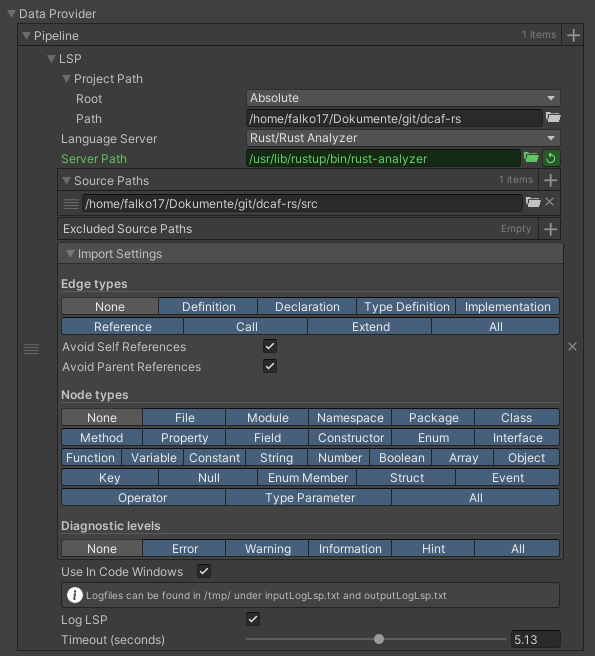
\includegraphics[width=0.95\textwidth]{unity_lsp_provider}
	\end{center}
	% Beware of sentences like the below, where all words except "for" and "the" are glossary terms.
	\caption{\gls{editor} \gls{ui} for the \gls{lsp} \gls{provider}}\label{fig:unity_lsp_provider}
\end{figure}

In that figure, we can see a configuration for the \tt{dcaf-rs} project\footnote{
	This is one of the sample projects we use in \cref{sec:techeval}'s technical evaluation.
}, where the \gls{ls} is the Rust Analyzer.
At the top, we can see that the path to the source project has been set, and that the \emph{Rust Analyzer}\footnote{
	The menu is grouped by language when opening it, hence the \texttt{Rust/} in front in \cref{fig:unity_lsp_provider}.
} has been selected as a \gls{ls}.
Below that, there is a field for "Source Paths".
This refers to the directories that shall be scanned for relevant documents, whereas a document's relevance is determined by its file extension.
This is distinct from the "Project Path" as that is instead used by the \gls{ls} to, for example, scan for project configuration files that describe dependencies.
Conversely, "Excluded Source Paths" can be used for those paths within the configured source paths that should be ignored (\eg, generated files, tests).

The selectable \glspl{ls} are only those that I have explicitly tested and confirmed to work with the algorithm---many servers are unusable, for example, due to required \glspl{capability} missing (such as the document symbols one).
All in all, there are working\footnote{
	There may well be more, I could not test some of the available \glspl{ls} either due to setup problems, or (like in the case of Wolfram Mathematica) because I do not have a license for the language in question.
} \glspl{ls} for the programming languages
C,
C++,
C\#,
Dart,
Go,
Haskell,
Java,
JavaScript,
Kotlin,
Lua,
MATLAB,
PHP,
Python,
Ruby,
Rust,
TypeScript,
and Zig.
There are also functioning \gls{ls} configurations for the miscellaneous languages
JSON,
\LaTeX{},
Markdown,
and XML.
A \gls{city} of a markup language like \LaTeX{}, for example, would have nodes for each section, figure, and so on, with edges representing references between these elements.

Next down the list in \cref{fig:unity_lsp_provider}, we have the import settings, which can be used to further refine the \gls{lsp}-generated data that is used for the project graph.
Specifically, we can select what kinds of nodes and edges we want to import, and which diagnostics we want to include.
Additionally, for the edges, there is the option to exclude loops and edges (not taking \tt{partOf} into account) to a node's direct parent.
The purpose behind this option is that otherwise, there are going to be a lot of definition/declaration edges from elements to their immediate parents, which happens because the locations returned by these \gls{lsp} functions often extend slightly outside the node's actual locations.
For example, a quirk of some \glspl{ls} is that a returned location may begin at \tt{\textcolor{red}{i}nt value}, while the actual node for this variable starts at \tt{int \textcolor{red}{v}alue}---in that case, the returned location would instead resolve to the outer container, such as the function it is contained in.

Finally, there is an option to enable the \gls{lsp} functions for \glspl{window} that are detailed in \cref{sec:intowindow}, a setting to generate log files for the transferred \gls{jrpc} messages, and a slider to adjust the maximum time we should wait for a \gls{ls}'s response to a request.
With all of these options configured, the graph can be loaded and drawn (and optionally exported to a \gls{gxl} file), where a bar displays the approximate progress of the process.
At this point, we will once again refer back to the explanatory video\footnote{\web{https://www.youtube.com/watch?v=yAzyv2\_q2ng}{2025-01-15}},
which goes over the implemented functionality in a bit more detail and may be easier to follow along than this textual description.
Some examples of \glspl{city} rendered using this algorithm are given in \cref{fig:gencities} in \cref{sec:techeval}.

\section{Integrating LSP Functionality into Code Cities}\label{sec:intocity}
After having examined how \glspl{city} are generated through the use of \gls{lsp}, we are now going to take a quick look at how some \gls{lsp} \glspl{capability} are integrated into \SEE{}.
For this section, we are going to purely focus on the interaction with the city itself, saving \glspl{window} for the following \cref{sec:intowindow}.

\subsection{Hover information}\label{subsec:hover}
The first thing I implemented was the functionality that, when hovering above nodes, the \gls{lsp} hover information should be displayed.
We already had an implementation for a tooltip that shows arbitrary text when hovering above nodes in \SEE{}, but I had to change it in two ways to work for this implementation:
\begin{enumerate}
	\item It is now a \gls{singleton} (since there will only be at most one tooltip per screen), making it easier to use as a caller.
	\item The tooltip now disappears when the user moves their mouse, and re-appears when the mouse is kept in place for a certain amount of time.
\end{enumerate}

\begin{figure}
	\begin{center}
		% l b r t
		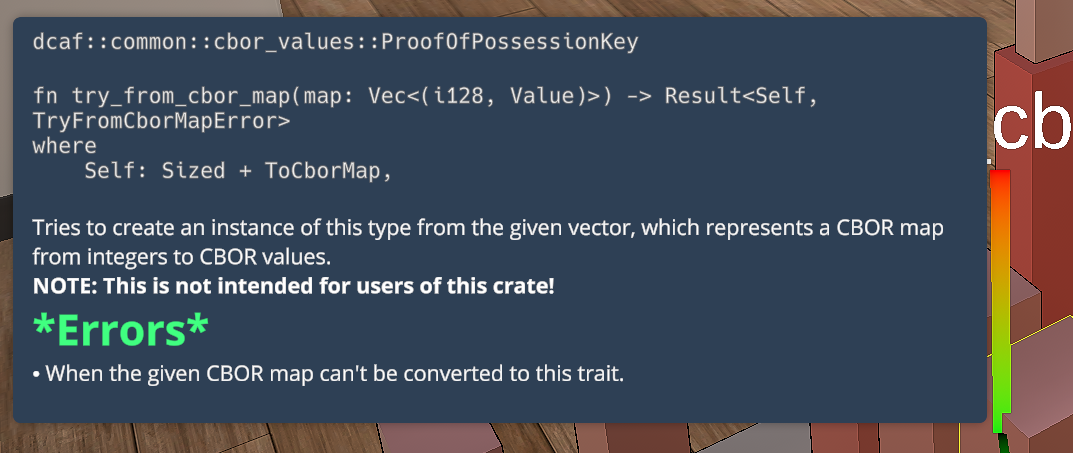
\includegraphics[trim={0.3cm 0.8cm 2.7cm 0.3cm},clip,width=0.95\textwidth]{HoverInfo}
	\end{center}
	\caption{A hover info tooltip with Markdown text converted to TextMeshPro rich text tags.}\label{fig:hoverinfo}
\end{figure}

Displaying the hover info is then relatively straightforward, as \cref{alg:generate} already saved it in the nodes of the city, so we need not even make any actual \gls{lsp} requests.
However, there is one more feature here that would be nice to support:
Some \glspl{ls} return the hover info as Markdown-formatted text instead of just plain text.
While Markdown by itself is still readable, we can leverage the XML-like rich text tags in Unity's TextMeshPro package\footnote{
	\web{http://digitalnativestudios.com/textmeshpro/docs/rich-text/}{2024-12-15}
} to display the Markdown text (partially, at least) in its proper formatting.
For this, I used the Markdig parser~\cite{mutel2024} and implemented a custom renderer to output the corresponding TextMeshPro tags.
An example for a "rich" hover info tooltip like this can be seen in \cref{fig:hoverinfo}.

\subsection{Context Menu Navigation}\label{subsec:citycontext}
While the various connections between nodes (\ie{}, references, definitions, etc.) can already visually be represented as edges in the scene, this is not always the most accessible option.
For example, in very large projects, the huge number of edges would make it very hard to discern individual connections, so edges are often excluded from the rendering.
Another problem with edges is that, as the evaluation will show (see \cref{subsec:comments}), it is sometimes hard to discern which node a certain edge points to.

\begin{minipage}[t]{.75\textwidth}
	\centering
	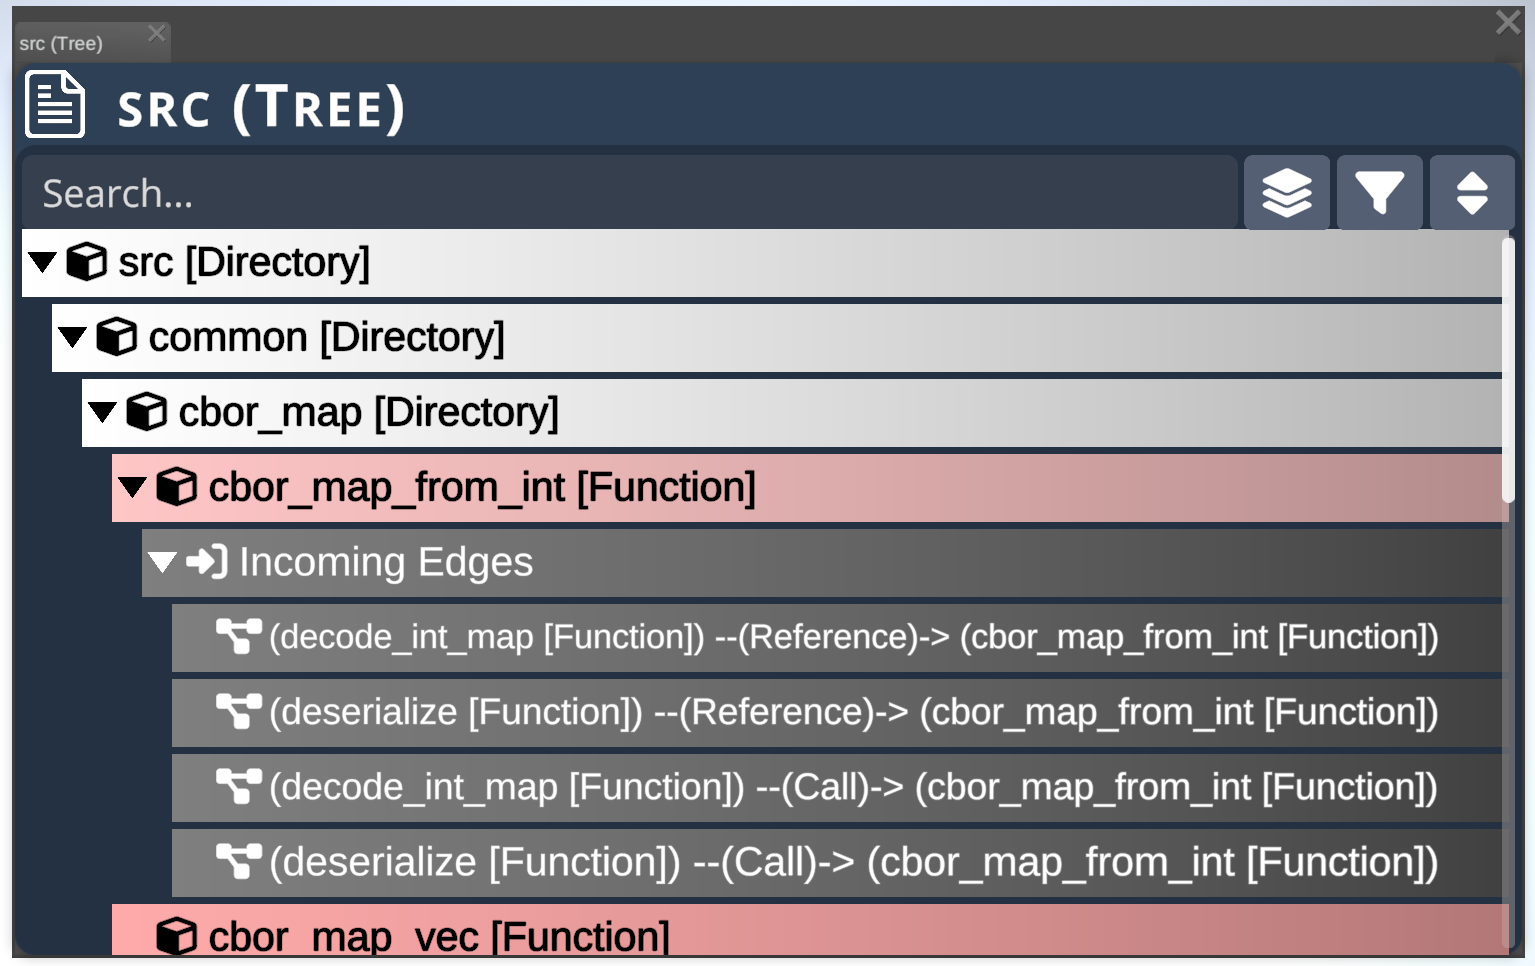
\includegraphics[width=0.97\textwidth]{TreeWindow}
	\captionof{figure}{The tree view for a \gls{city} in \SEE{}.}\label{fig:treeview}
\end{minipage}%
\begin{minipage}[t]{.25\textwidth}
	\captionsetup{format=plain}
	\centering
	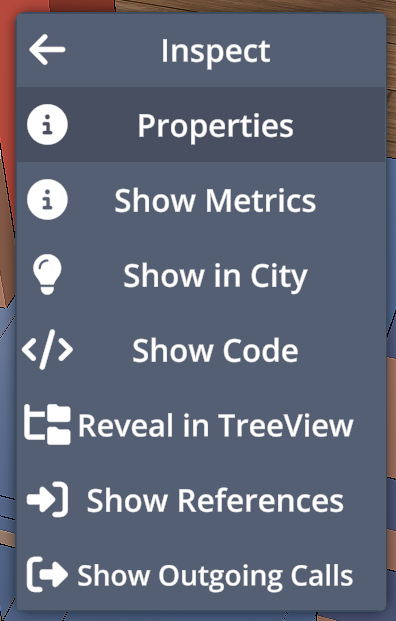
\includegraphics[width=0.9\textwidth]{CityContextMenu}
	\captionof{figure}{Context menu options for a node in an \gls{lsp}-enabled \gls{city}.}\label{fig:contextcity}
\end{minipage}

For cases like that, users could open the tree view for the city, which is a hierarchical 2D representation of the project graph that also shows the outgoing and incoming edges for each node (see \cref{fig:treeview}).
However, although it is useful, it is still cumbersome to look around in the city and to then have to open this tree view and navigate around in it to find out what a certain node is connected to.
The context menu seems like a fitting place to remedy this:
Right-clicking a node opens a menu that is shown in \cref{fig:contextcity} with several actions, such as opening the tree view for this node or opening its \gls{window}.
As part of the implementation here, the context menu will now also display \gls{lsp} navigation entries such as "Show outgoing calls," given that corresponding edges exist.
Clicking on this entry leads to one of two things happening:
\begin{itemize}
	\item If there is only one target, it will be immediately highlighted with a spear and glow to make it easily identifiable in the scene.\footnote{
		      Once again, I recommend watching \href{https://www.youtube.com/watch?v=yAzyv2_q2ng}{the showcase video} to see this effect in action.
	      }
	\item If there is more than one target, a modified tree view will open, containing only the targets of the edge.
	      The user can click on one of the results here to trigger the highlighting described above.
\end{itemize}

\subsection{Diagnostics as Erosion Icons}
Finally, we are displaying \gls{lsp}-sourced diagnostics as erosion icons above each node.
As described in \cref{sec:generate} and specifically \cpageref{alg:generate:end3,alg:generate:funcend} of \cref{alg:generate}, we retrieve these diagnostics either by using the pull diagnostics \gls{capability} if it is available, or we collect pushed diagnostics during the import process.
We then associate diagnostics to nodes using the \gls{intervaltree}-based function described in \cref{subsec:kd}.
Finally, if the user enabled this in the configuration, we aggregate diagnostics upwards so that collected diagnostics can also be seen on the module they are in, for example.

We are not going to go into the details of the rendering and display of the nodes, as this just re-uses the same mechanisms as the implementation from my bachelor's thesis~\cite[section~3.3]{galperin2021}.
There were only minimal changes, like the integration of new icons for the different \gls{lsp} diagnostic types, and a change that allows leaf erosion icons to be displayed on non-leaf nodes, since the \gls{lsp} diagnostics are not always present at the lowest level in the hierarchy.

\section{Integrating LSP Functionality into Code Windows}\label{sec:intowindow}
Now we will go over how the functionalities of \glspl{ls} have been integrated into \glspl{window} to make them more \gls{ide}-like.
Some of these functionalities will seem quite similar to the way the corresponding \gls{city} \gls{lsp} features were implemented in the previous section.
However, a crucial difference here is that, for \glspl{city}, the pre-computed \gls{lsp} attributes from \cref{alg:generate} are used (\ie, no actual requests are made to the \gls{ls}, it does not even have to be running), while for \glspl{window}, all \gls{lsp} functionality does actually go through the \gls{ls} as a proper \gls{jrpc} request.
\Cref{fig:lspwindow} showcases what a \gls{window} with the newly added \gls{lsp} features looks like.

\begin{figure}
	\begin{center}
		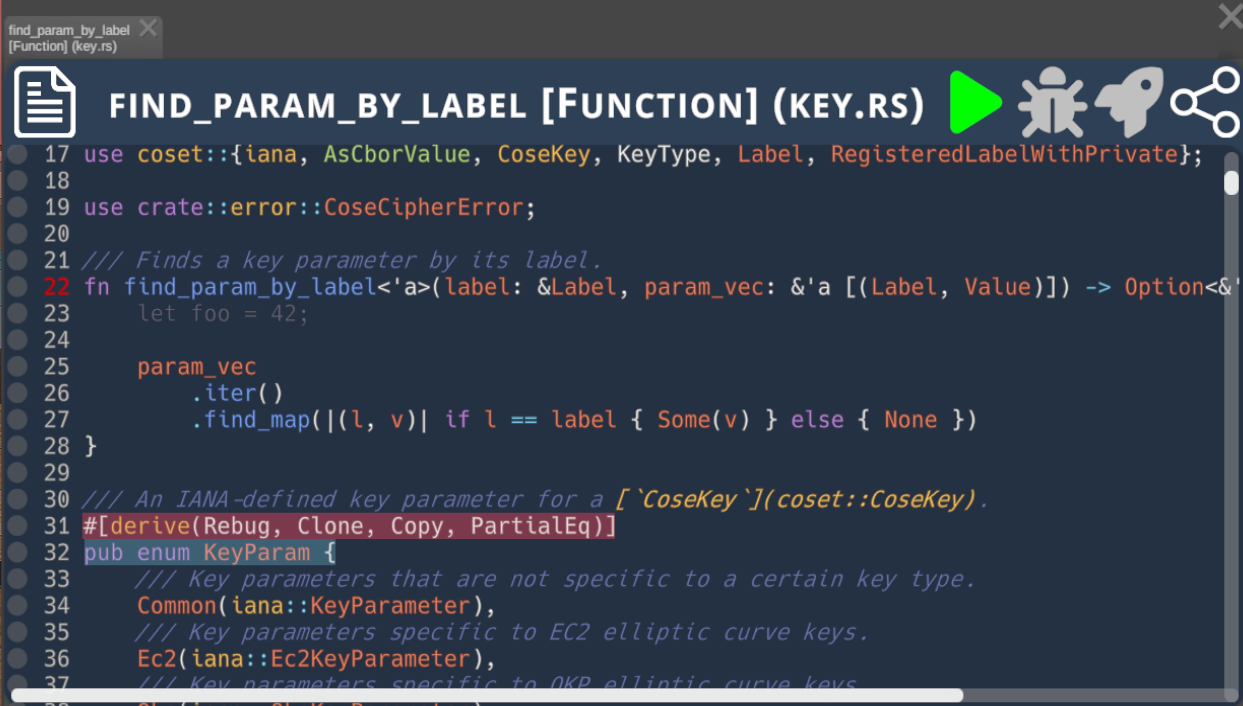
\includegraphics[width=0.95\textwidth]{CodeWindow}
	\end{center}
	\caption{A \gls{window} with enabled \gls{lsp} integration.}\label{fig:lspwindow}
\end{figure}

\subsection{Syntax Highlighting}
\SEE{} already has support for syntax highlighting using Antlr-generated lexers, which works by converting the token stream returned by the lexer into a string of TextMeshPro rich text, as for the hover info in \cref{subsec:hover}.
The rich text then contains color tags that render each element in the desired color.
This implementation was very heavily coupled to Antlr and the token types it offers, so some larger refactoring was necessary to abstract over both Antlr and \gls{lsp} as a token source.
Retrieving \gls{lsp} tokens also required a bit more scaffolding code (\eg, semantic tokens are not always immediately available when opening the file, making it necessary to poll the \gls{ls} until the tokens are ready), and I noticed some bugs with the way the existing syntax highlighting was implemented into the \glspl{window}.
Also, the semantic tokens returned by the \gls{ls} uses a very compact encoding, consisting of only a list of integers that decode to token types along with positions relative to the previous token~\cite{lsp}---since the \glspl{window} need absolute positions to be able to determine the start and end of the rich text tags instead, another decoding and conversion\footnote{
	Yet \emph{another} issue was the fact that semantic tokens, in contrast to Antlr tokens, do not cover the whole document (\eg, there are no token types for whitespace), so we have to read through the document while iterating over the semantic tokens to construct the final set of tokens that can be used by the \glspl{window}.
} step was necessary here.
Finally, support for token modifiers---a concept exclusive to semantic tokens---had to be added.
I decided on the following mapping from modifiers\footnote{
	There are more modifiers than this, such as one for asynchronous code, but at this point I ran out of available (and reasonable) rich text tags.
} to rich text tags (in accordance to how \glspl{ide} usually handle this):
\begin{itemize}
	\item Static elements and documentation are rendered in \textit{italic text}.
	\item Deprecated elements are rendered in \st{strikethrough text}.
	\item Variables that are modified are rendered in \underline{underlined text}.
\end{itemize}

Due to all of this making it quite a bit more complicated to support semantic tokens than I first thought, this is where most of the effort and changed lines referenced in the row for the corresponding pull request in \cref{tab:code} went,
so subsequent subsections shall seem shorter and substantially simpler.

\subsection{Hover information}
Implementing the hover functionality was fairly straightforward, as it has already been implemented for \glspl{city}.
The only thing I had to work around was that, within Unity, I could only get the byte offset of the clicked character within the text as a whole, while the \gls{lsp} hover information can only be queried for a two-dimensional \gls{range}.
To fix this without sacrificing too much performance, we have to maintain a mapping from line numbers to the "global" offset of the newline character, which we can then use to convert from a global offset to a \gls{range}.

\subsection{Diagnostic Highlighting}
Highlighting diagnostics in the \glspl{window} was already implemented with the Axivion Dashboard as a source, so
similar to the semantic tokens, I had to implement an abstraction over diagnostics' sources, although this was much easier than abstracting over token sources.
Diagnostics show up in two ways in the \glspl{window}:
By highlighting the corresponding code range in a color corresponding to the type of diagnostic, and by providing the diagnostic's content when hovering over that code range (both of these were already implemented for my bachelor's thesis~\cite{galperin2021}).
I modified the hover text to indicate the source of the diagnostic and added special handling for the "element unused" diagnostic to render the text in grey, as is done in many \glspl{ide}.
The rest just involved mapping the \gls{lsp} diagnostics' offset to the global offset in order to insert the rich text tags that highlight the code range at the correct position.
We can see three example diagnostics in \cref{fig:lspwindow} in lines 23, 31, and 32, respectively.

\subsection{Navigation}

\begin{figure}
	\centering
	\begin{subfigure}{0.47\textwidth}
		
\includegraphics[width=\textwidth]{CodeWindowContext}
		\caption{The context-menu that is shown when right-clicking an element.}\label{fig:windowcontext}
	\end{subfigure}
	\begin{subfigure}{0.47\textwidth}
		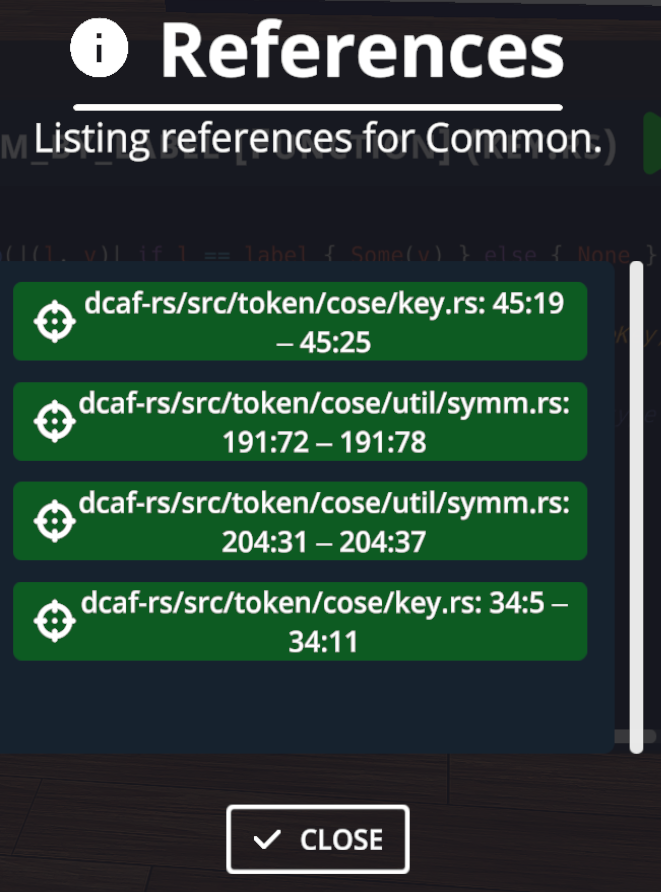
\includegraphics[width=\textwidth]{CodeWindowReferences}
		\caption{Menu from which the user can select an \gls{lsp} reference to navigate to.}\label{fig:windowmenu}
	\end{subfigure}
	\caption{Navigation features in an \gls{lsp}-enabled \gls{window}.}\label{fig:windownav}
\end{figure}


Similar to \cref{subsec:citycontext}, I added the ability to right-click code elements and open a context menu with various navigation options, such as "go to definition," or "show references" (see \cref{fig:windowcontext}).
Taking "show references" as an example, if there are multiple targets, a dialog is shown in which the references are shown as a list of files along with their ranges, as in \cref{fig:windowmenu}.
The user can then select one of these ranges.
This step is skipped if there is only a single target.
After selecting a reference, if it belongs to the current file, the range is simply scrolled into view and the corresponding line is highlighted, otherwise a new \gls{window} (or an existing one, if the file is already open elsewhere) is opened first.
While implementing this, I also noticed a bug in the OmniSharp \gls{lsp} library that causes the call hierarchy request to fail, so I implemented a workaround and submitted an issue.\footnote{
	\web{https://github.com/OmniSharp/csharp-language-server-protocol/issues/1303}{2024-12-27}
}

As an additional feature copied from popular \glspl{ide}, it is possible to hold down \keystroke{Ctrl} and then click on an element in the \gls{window}, which has the same effect as right-clicking that word first and then selecting "Go to definition".
This is useful because it allows the user to quickly jump to the definition of, for example, a function to find out its content, which is a very common operation.

\section{Technical Evaluation}\label{sec:techeval}
Before ending this chapter, we want to briefly evaluate the implementation on a technical level.
While there are some unit tests for parts of the algorithm, taking real-world projects and trying to generate \glspl{city} out of them using our implementation is important to verify that it is working correctly too.
Apart from a quick qualitative glance at each generated city, we are also interested in an analysis of performance here---we made quite a few theoretical statements and analyses in \cref{sec:generate}, so we can also use this section to make sure the \gls{intervaltree}-based \cref{alg:interval} actually does work more efficiently than the original "brute-force" approach of \cref{alg:generate}.

I ran the city generation algorithm on the following projects:
\begin{itemize}
	\item \textbf{JabRef}~\cite{jabref}: A bibliography manager written in Java.
	\item \textbf{SpotBugs}~\cite{spotbugs}: A bug-detector using static analysis for Java code.
	\item \textbf{\proptt{dcaf-rs}}~\cite{dcaf}: A Rust project about authentication in the Internet of Things.
	\item \textbf{\proptt{aaoffline}}~\cite{aaoffline}: A Rust downloader for a certain kind of online mystery game.
	\item \textbf{\LaTeX{} source of this master's thesis}\footnote{
		      I could not use the whole content of the thesis---for example, it would have been difficult to include the results of the technical evaluation while I was still in the process of collecting them.
		      See \cref{app:source}.
	      }: Self-explanatory.
	\item \textbf{\LaTeX{} source of my bachelor's thesis}: Self-explanatory.
\end{itemize}

The algorithm was repeated three times for the first two projects and five times for the others\footnote{
	The difference stems from the fact that the generation for JabRef and SpotBugs took much longer.
}, to make sure that any single result was not an outlier.
For the generation, we enabled every edge type, node type, and diagnostic, except for JabRef and SpotBugs, where we only enabled some node types (namely File, Module, Namespace, Package, Class, and Interface) and only one edge type (Extend for JabRef and Reference for SpotBugs), otherwise the generation would have taken much too long.
\Cref{tab:benchmark} lists all projects along with their node count, edge count, \gls{loc}, and average generation time.

\begin{table*}[htbp]
	\caption{Relevant metadata for all evaluated projects, along with the average total generation time.}\label{tab:benchmark}
	\begin{tabular}{@{}llccccc@{}}
		\toprule
		\multicolumn{1}{c}{\multirow{2}{*}{\textbf{Name}}} & \multicolumn{1}{c}{\multirow{2}{*}{\textbf{\Gls{ls}}}} & \multicolumn{1}{c}{\multirow{2}{*}{\textbf{k\gls{loc}}}} & \multicolumn{1}{c}{\multirow{2}{*}{\textbf{\# Nodes}}} & \multicolumn{1}{c}{\multirow{2}{*}{\textbf{\# Edges}}} & \multicolumn{2}{c}{\textbf{Average Time [h:m]}}                         \\
		                                                   &                                                        &                                                          &                                                        &                                                        & {Optimized}                                     & {Brute-force}         \\
		\midrule
		\textit{JabRef}                                    & Eclipse JDT                                            & $\num{179}$                                              & $\num{5575}$                                           & $\num{919}$                                            & $4$:$\num{17}$                                  & $4$:$\num{29}$        \\
		\textit{SpotBugs}                                  & Eclipse JDT                                            & $\num{216}$                                              & $\num{3813}$                                           & $\num{16262}$                                          & $9$:$\num{22}$                                  & $\num{43}$:$\num{11}$ \\
		\textit{\proptt{dcaf-rs}}                          & Rust Analyzer                                          & $\num{16}.5$                                             & $\num{1192}$                                           & $\num{9940}$                                           & $4$:$\num{27}$                                  & $5$:$\num{59}$        \\
		\textit{\proptt{aaoffline}}                        & Rust Analyzer                                          & $3.3$                                                    & $\num{515}$                                            & $\num{1250}$                                           & $0$:$\num{46}$                                  & $0$:$\num{56}$        \\
		\textit{Master's thesis}                           & \proptt{texlab}                                        & $2.5$                                                    & $\num{301}$                                            & $\num{24048}$                                          & $0$:$\num{10}$                                  & $0$:$\num{36}$        \\
		\textit{Bachelor's thesis}                         & \proptt{texlab}                                        & $2$                                                      & $\num{376}$                                            & $\num{46348}$                                          & $0$:$\num{13}$                                  & $2$:$\num{31}$        \\ \bottomrule
	\end{tabular}
\end{table*}

The first thing that is worth mentioning here is that generations by different \glspl{ls} are not really comparable to one another.
For example, we can see that the generation run for this thesis took on average ten seconds---faster than any other project---even though there were more edges than in almost every other project.
This difference cannot be explained by the idea that edges may not play a big role in generation time after all, since a closer look at the data for JabRef and SpotBugs reveals a much longer generation time for SpotBugs, even though SpotBugs has less nodes (but a lot more edges) than JabRef.
Hence, the difference there has to come from the different \glspl{ls}.
This is also why we have chosen to analyze two projects per \gls{ls}.

We can already make two observations from \cref{tab:benchmark}:
The more edges there are, the more time the generation takes (again, only within the same language), and the brute-force version always takes longer than the optimized version.
To examine these claims in more detail, I have created some bar graphs comparing the average generation time in \cref{fig:techeval}.
There, the optimized version (suffix $O$) is compared against the brute-force version (suffix $B$), and the runtime of the algorithm is broken down by its components:
\begin{itemize}
	\item \textbf{Nodes} refers to part I of the algorithm (\crefrange{alg:generate:begin}{alg:generate:end1}),
	\item \textbf{Tree Creation} refers to the construction of the augmented \gls{intervaltree},
	\item \textbf{Edges} refers to part II of the algorithm (\crefrange{alg:generate:end1}{alg:generate:end2}),
	\item \textbf{Diagnostics} refers to collecting and handling the diagnostics (\cref{alg:generate:diag}),
	\item \textbf{Aggregation} refers to the upward aggregation of metrics (\crefrange{alg:generate:agg}{alg:generate:end3}), and finally,
	\item \textbf{Miscellaneous} consists of the timespans outside of the measured ranges (\eg, collecting documents).
\end{itemize}

% Visualizations / Analyses:
% - Taking a look at the city itself, making sure it looks right.
% - What I want to show:
%   ✓ Normal running time vs optimized running time.
%   ✓ Running time of various parts of the algorithm (in percent?)
%   ✓ Advantage of optimized over brute force compared to num edges!
% - Maybe Stacked Bar Chart for time components per system?

\begin{figure}
	\begin{subfigure}[T]{0.5\textwidth}
		\begin{center}
			\begin{tikzpicture}
				\begin{axis}[
						ylabel={Time in seconds},
						height=10cm,
						ybar stacked,
						name=bars,
						set layers,
						ymin=0, ymax=370,
						axis line style={draw=none},
						enlarge x limits={0.5},
						ymajorgrids,
						bar width=0.6cm,
						x tick label style={rotate=45, anchor=east, align=left, font=\scriptsize, yshift=-2},
						xtick=data,
						width=\textwidth,
						xticklabels={\proptt{aaoffline}-$O$, \proptt{aaoffline}-$B$, \proptt{dcaf-rs}-$O$, \proptt{dcaf-rs}-$B$},
						xtick={0,1,3,4},
					]

					\addplot+[fill] table [x=index,y=LSP Nodes,col sep=tab] {benchmark/rust.dat};
					\addplot+[fill] table [x=index,y=LSP Edges,col sep=tab] {benchmark/rust.dat};
					\addplot+[fill] table [x=index,y=LSP Diagnostics,col sep=tab] {benchmark/rust.dat};
					\addplot+[fill] table [x=index,y=LSP Aggregate,col sep=tab] {benchmark/rust.dat};
					\addplot+[fill] table [x=index,y=LSP Tree,col sep=tab] {benchmark/rust.dat};
					\addplot+[fill] table [x=index,y=LSP Miscellaneous,col sep=tab] {benchmark/rust.dat};
				\end{axis}
				\plotornaments{bars}
			\end{tikzpicture}
		\end{center}
	\end{subfigure}
	\begin{subfigure}[T]{0.5\textwidth}
		\begin{center}
			\begin{tikzpicture}
				\begin{axis}[
						height=10cm,
						ybar stacked,
						name=bars,
						set layers,
						ymin=0, ymax=155,
						axis line style={draw=none},
						enlarge x limits={0.5},
						ymajorgrids,
						bar width=0.6cm,
						x tick label style={rotate=45, anchor=east, align=left, font=\scriptsize, yshift=-2},
						xtick=data,
						width=\textwidth,
						xticklabels={Bachelor-$O$, Bachelor-$B$, Master-$O$, Master-$B$},
						xtick={0,1,3,4},
						legend entries={Nodes, Edges, Diagnostics, Aggregation, Tree Creation, Miscellaneous},
						legend style={nodes={scale=0.7, transform shape}, at={(0.95,0.9)}}
					]

					\addplot+[fill] table [x=index,y=LSP Nodes,col sep=tab] {benchmark/tex.dat};
					\addplot+[fill] table [x=index,y=LSP Edges,col sep=tab] {benchmark/tex.dat};
					\addplot+[fill] table [x=index,y=LSP Diagnostics,col sep=tab] {benchmark/tex.dat};
					\addplot+[fill] table [x=index,y=LSP Aggregate,col sep=tab] {benchmark/tex.dat};
					\addplot+[fill] table [x=index,y=LSP Tree,col sep=tab] {benchmark/tex.dat};
					\addplot+[fill] table [x=index,y=LSP Miscellaneous,col sep=tab] {benchmark/tex.dat};
				\end{axis}
				\plotornaments{bars}
			\end{tikzpicture}
		\end{center}
	\end{subfigure}\\
	\begin{subfigure}[T]{0.5\textwidth}
		\begin{center}
			\begin{tikzpicture}
				\begin{axis}[
						ylabel={Time in seconds},
						height=10cm,
						ybar stacked,
						name=bars,
						set layers,
						ymin=0, ymax=280,
						xmin=0, xmax=1,
						axis line style={draw=none},
						enlarge x limits={1},
						ymajorgrids,
						bar width=0.6cm,
						x tick label style={rotate=45, anchor=east, align=left, font=\scriptsize, yshift=-2},
						xtick=data,
						width=\textwidth,
						xticklabels={JabRef-$O$, JabRef-$B$},
						xtick={0,1},
					]

					\addplot+[fill] table [x=index,y=LSP Nodes,col sep=tab] {benchmark/java.dat};
					\addplot+[fill] table [x=index,y=LSP Edges,col sep=tab] {benchmark/java.dat};
					\addplot+[fill] table [x=index,y=LSP Diagnostics,col sep=tab] {benchmark/java.dat};
					\addplot+[fill] table [x=index,y=LSP Aggregate,col sep=tab] {benchmark/java.dat};
					\addplot+[fill] table [x=index,y=LSP Tree,col sep=tab] {benchmark/java.dat};
					\addplot+[fill] table [x=index,y=LSP Miscellaneous,col sep=tab] {benchmark/java.dat};
				\end{axis}
				\plotornaments{bars}
			\end{tikzpicture}
		\end{center}
	\end{subfigure}
	\begin{subfigure}[T]{0.5\textwidth}
		\begin{center}
			\begin{tikzpicture}
				\begin{axis}[
						height=10cm,
						ybar stacked,
						name=bars,
						set layers,
						ymin=0, ymax=2700,
						axis line style={draw=none},
						axis y line*=left,
						xmin=3, xmax=4,
						enlarge x limits={1},
						ymajorgrids,
						bar width=0.6cm,
						x tick label style={rotate=45, anchor=east, align=left, font=\scriptsize, yshift=-2},
						xtick=data,
						width=\textwidth,
						xticklabels={SpotBugs-$O$, SpotBugs-$B$},
						xtick={3,4},
					]

					\addplot+[fill] table [x=index,y=LSP Nodes,col sep=tab] {benchmark/java.dat};
					\addplot+[fill] table [x=index,y=LSP Edges,col sep=tab] {benchmark/java.dat};
					\addplot+[fill] table [x=index,y=LSP Diagnostics,col sep=tab] {benchmark/java.dat};
					\addplot+[fill] table [x=index,y=LSP Aggregate,col sep=tab] {benchmark/java.dat};
					\addplot+[fill] table [x=index,y=LSP Tree,col sep=tab] {benchmark/java.dat};
					\addplot+[fill] table [x=index,y=LSP Miscellaneous,col sep=tab] {benchmark/java.dat};
				\end{axis}
				\plotornaments{bars}
			\end{tikzpicture}
		\end{center}
	\end{subfigure}
	\caption{Generation time for each project, broken down by parts of the algorithm.
		The suffix \emph{O} denotes the optimized (\gls{intervaltree}) version of the algorithm, while \emph{B} refers to the brute-force version.
	}\label{fig:techeval}
\end{figure}

The generation of edges is by far the most expensive part\footnote{
	As the distribution of other components is hard to tell due to the edge component taking up so much space, there is another version of the diagram without this component in \cref{app:noedge}.
} of the algorithm, partly confirming our theoretical analysis from \cref{subsec:performance}.
The one exception to this seems to be JabRef, where the most expensive component consists of nodes.
This can be explained by the respective counts of the graph elements:
Because we only selected "Extend" edges for JabRef, it has the fewest edges out of all the projects ($919$) while having the most nodes out of all the projects ($5575$).
Another thing to note is that the only components big enough to even make out on the diagram are the node synthesis, the edge synthesis, and the collection of diagnostics (but not the aggregation), with the latter probably taking some time because it also makes use of the \textsc{FindNodesByLocation} function.

The optimized version of the algorithm is also always quicker than the brute-force version, and we can hypothesize based on these bar graphs that the relative improvement of the optimized version (\ie, the percentage by which time decreases when switching to the optimized version) over the number of edges is strictly monotonic, that is, the more edges there are, the more the optimized algorithm will shorten the total runtime in relation to the brute-force version.
We can check this hypothesis by plotting the relative time improvement as defined here against the number of edges in each project.

\begin{figure}
	\begin{center}
		\tikzexternaldisable
		\begin{tikzpicture}[
				labelnode/.style={font=\footnotesize,Maroon}
			]
			\begin{semilogxaxis}[
					height=9cm,
					name=line,
					set layers,
					ymin=0, ymax=1,
					xmin=10^(2.7), xmax=55000,
					xtick distance=10^(0.5),
					xtick distance=10^(0.5),
					axis line style={draw=none},
					grid=major,
					xlabel={Number of edges},
					ylabel={Relative time improvement},
					width=\textwidth,
				]

				\addplot+[draw=black,
					mark=*,
					mark options={fill=Maroon,draw=Maroon},
					% nodes near coords,
					% nodes near coords align={above left},
					% every node near coord/.append style={font=\footnotesize,Maroon},
					point meta=explicit symbolic,
					ultra thick,
					error bars/.cd,
					y dir=both,y explicit,
				] table [meta=project,x=edges,y=adv_mean,y error minus=adv_min,y error plus=adv_max,col sep=tab] {benchmark/advantage.dat};


				\node[labelnode] at (axis cs: 10^2.87,0.08) {JabRef};
				\node[labelnode] at (axis cs: 10^2.97,0.29) {\proptt{aaoffline}};
				\node[labelnode] at (axis cs: 10^3.9,0.29) {\proptt{dcaf-rs}};
				\node[labelnode] at (axis cs: 10^4.1,0.82) {SpotBugs};
				\node[labelnode] at (axis cs: 10^4.4,0.69) {Master's thesis};
				\node[labelnode] at (axis cs: 10^4.45,0.95) {Bachelor's thesis};
			\end{semilogxaxis}
			\plotornaments{line}
		\end{tikzpicture}
		\tikzexternalenable
	\end{center}
	\caption{The relative improvement of the optimized algorithm by number of edges (\ie, the percentage by which the time is reduced when using \cref{alg:interval} instead of the base \cref{alg:generate}).
		Error bars are only shown when their extent exceeds the diameter of the point, and describe the full range of datapoints (\ie, from minimum to maximum).
		\emph{Note the logarithmic x-axis.}
	}\label{fig:relimprov}
\end{figure}

\Cref{fig:relimprov} shows exactly that plot, but it disproves this hypothesis:
While almost every datapoint does seem to follow this rule, the relative time improvement for the master's thesis source code is actually lower than for SpotBugs, even though SpotBugs has fewer edges.
I suspect that the hypothesis is still directionally correct (the more edges there are, the more the optimization helps), but that it does not hold when making comparisons across multiple \glspl{ls}, since the performance differences between their implementation makes too big a dent.
The final thing to note from this plot is that, across all our samples, the brute-force version is never better than the optimized version of the algorithm, which we can tell by the fact that the error bars (denoting the minimum and maximum relative time improvement across all samples) never extend into the negatives.

\begin{figure}
	\begin{subfigure}{0.5\textwidth}
		\centering
		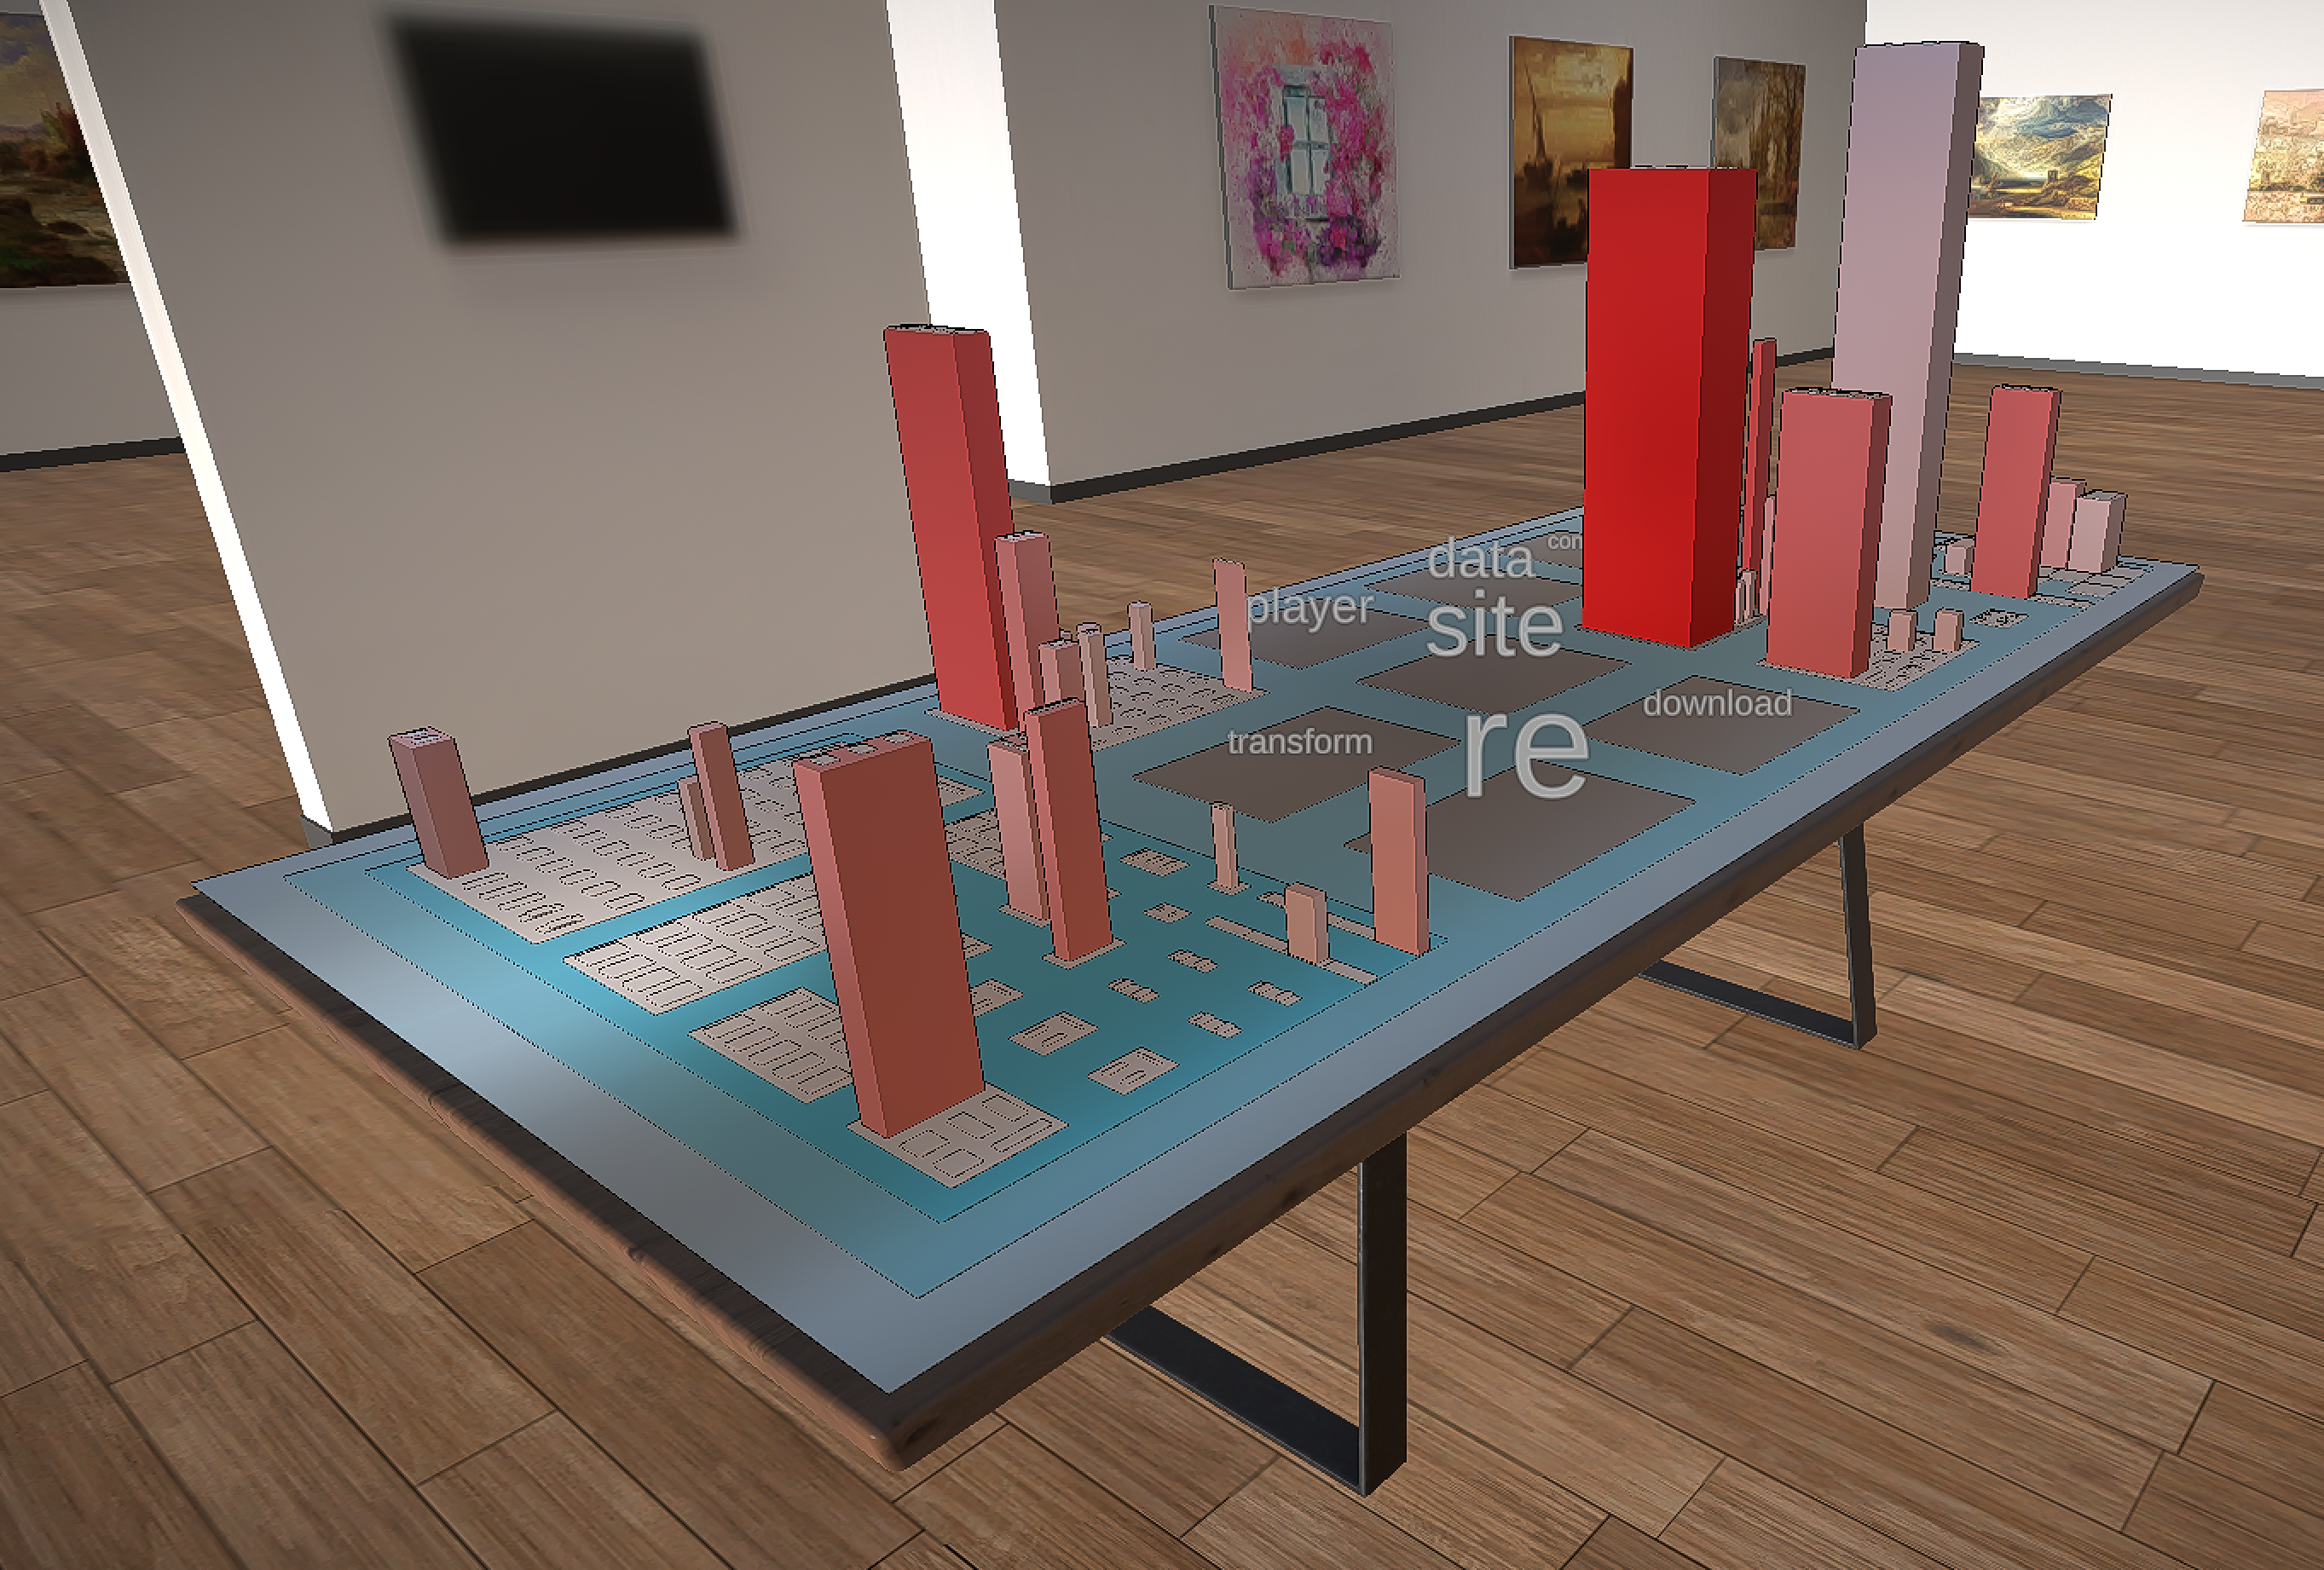
\includegraphics[width=\textwidth]{AaoCity}
		\caption{\Gls{city} for the \proptt{aaoffline} project.}\label{fig:aaocity}
	\end{subfigure}
	\begin{subfigure}{0.5\textwidth}
		\centering
		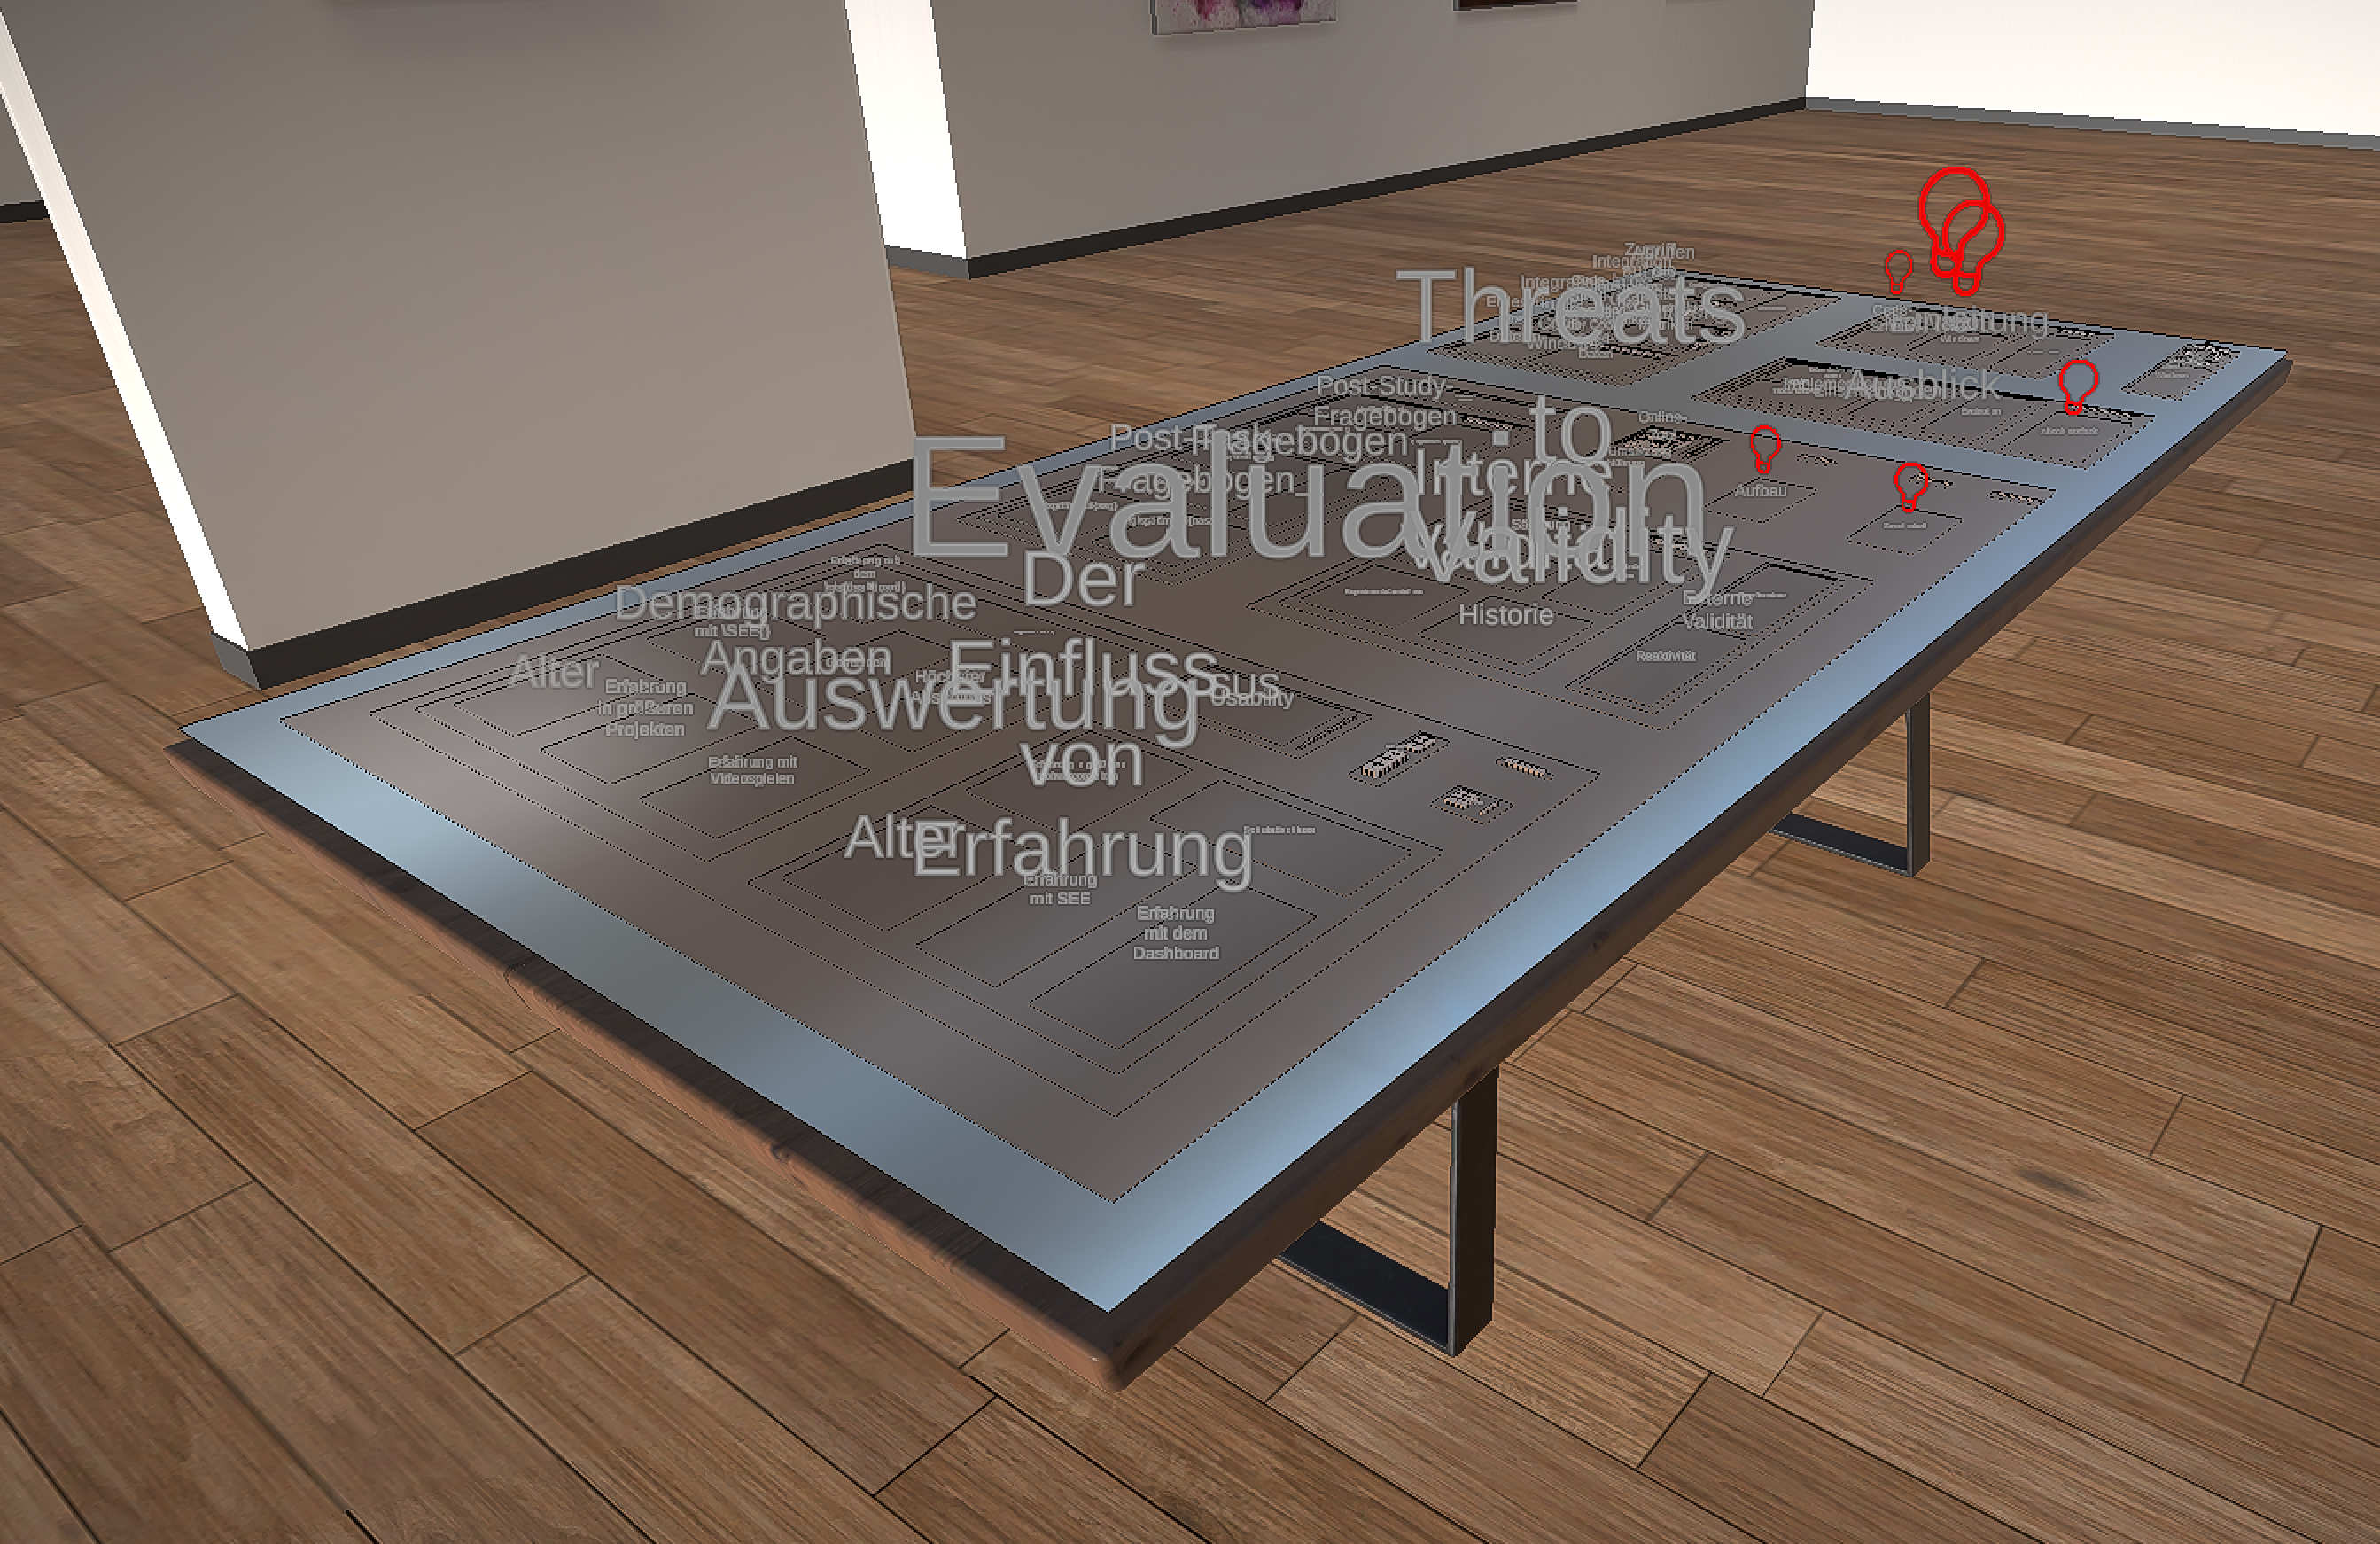
\includegraphics[width=\textwidth]{BachelorCity}
		\caption{\Gls{city} for my bachelor's thesis.}\label{fig:bachcity}
	\end{subfigure}
	\begin{subfigure}{0.5\textwidth}
		\centering
		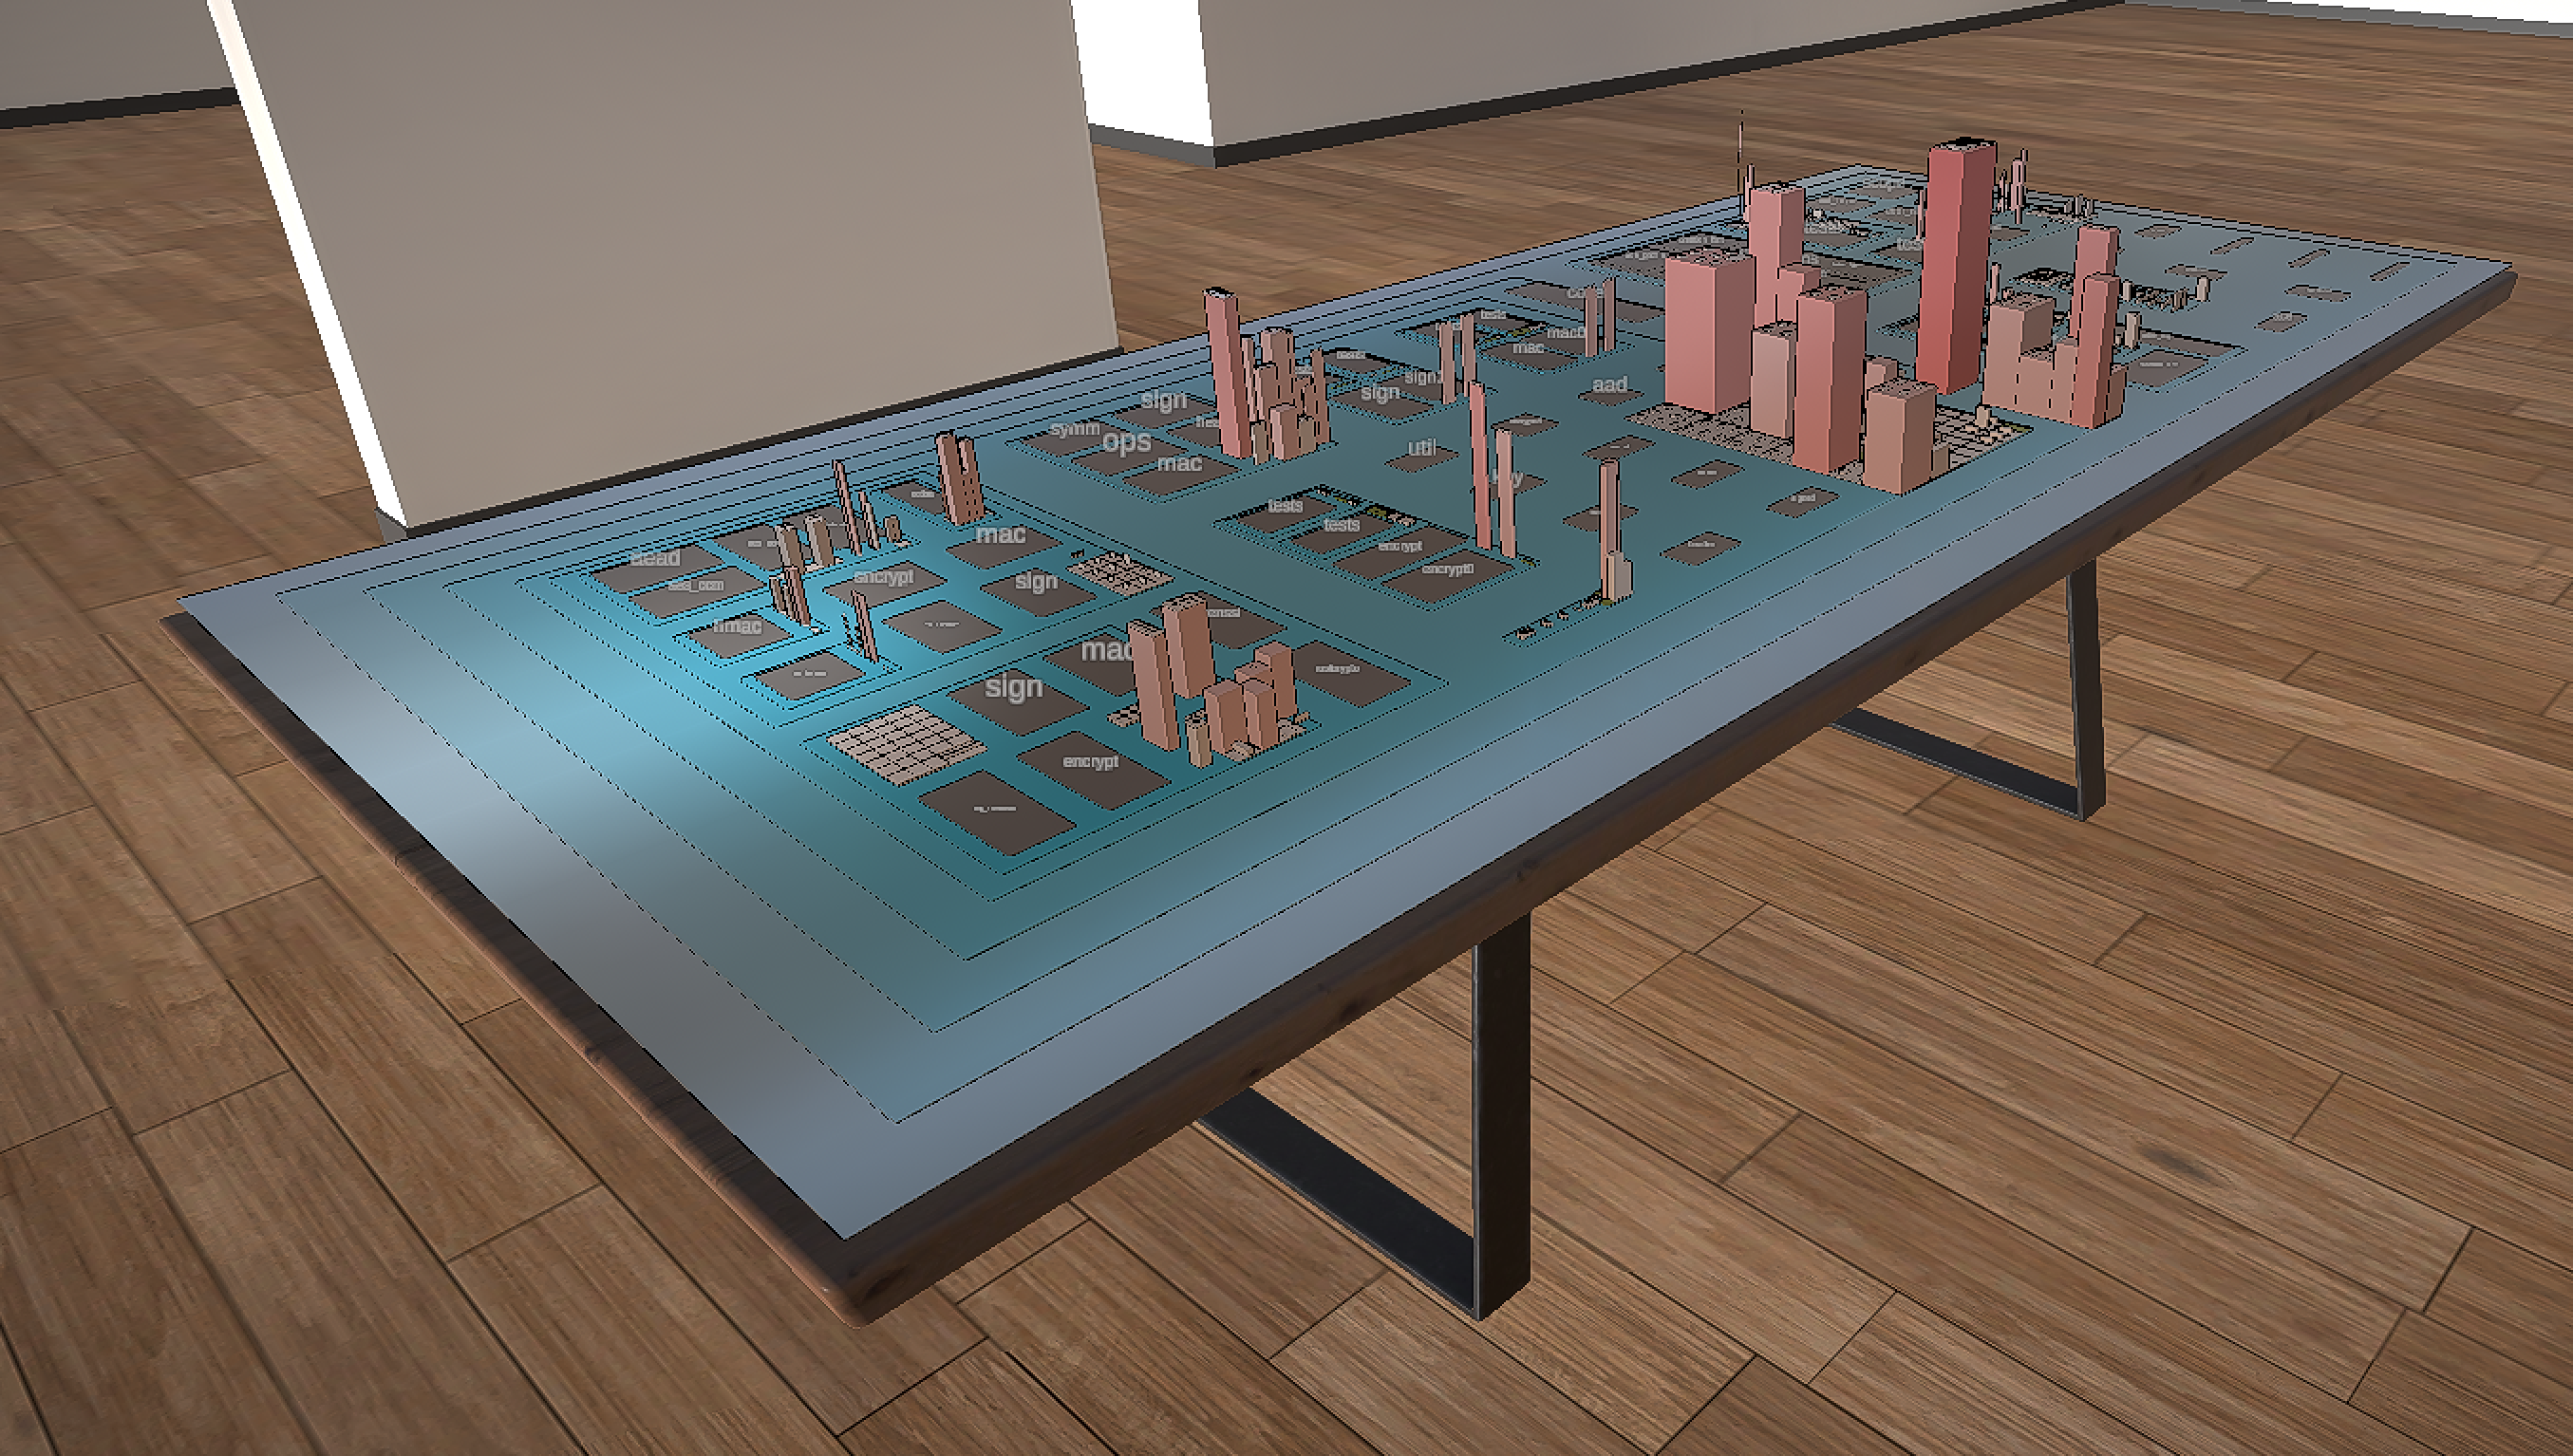
\includegraphics[width=\textwidth]{DcafCity}
		\caption{\Gls{city} for the \proptt{dcaf-rs} project.}\label{fig:dcafcity}
	\end{subfigure}
	\begin{subfigure}{0.5\textwidth}
		\centering
		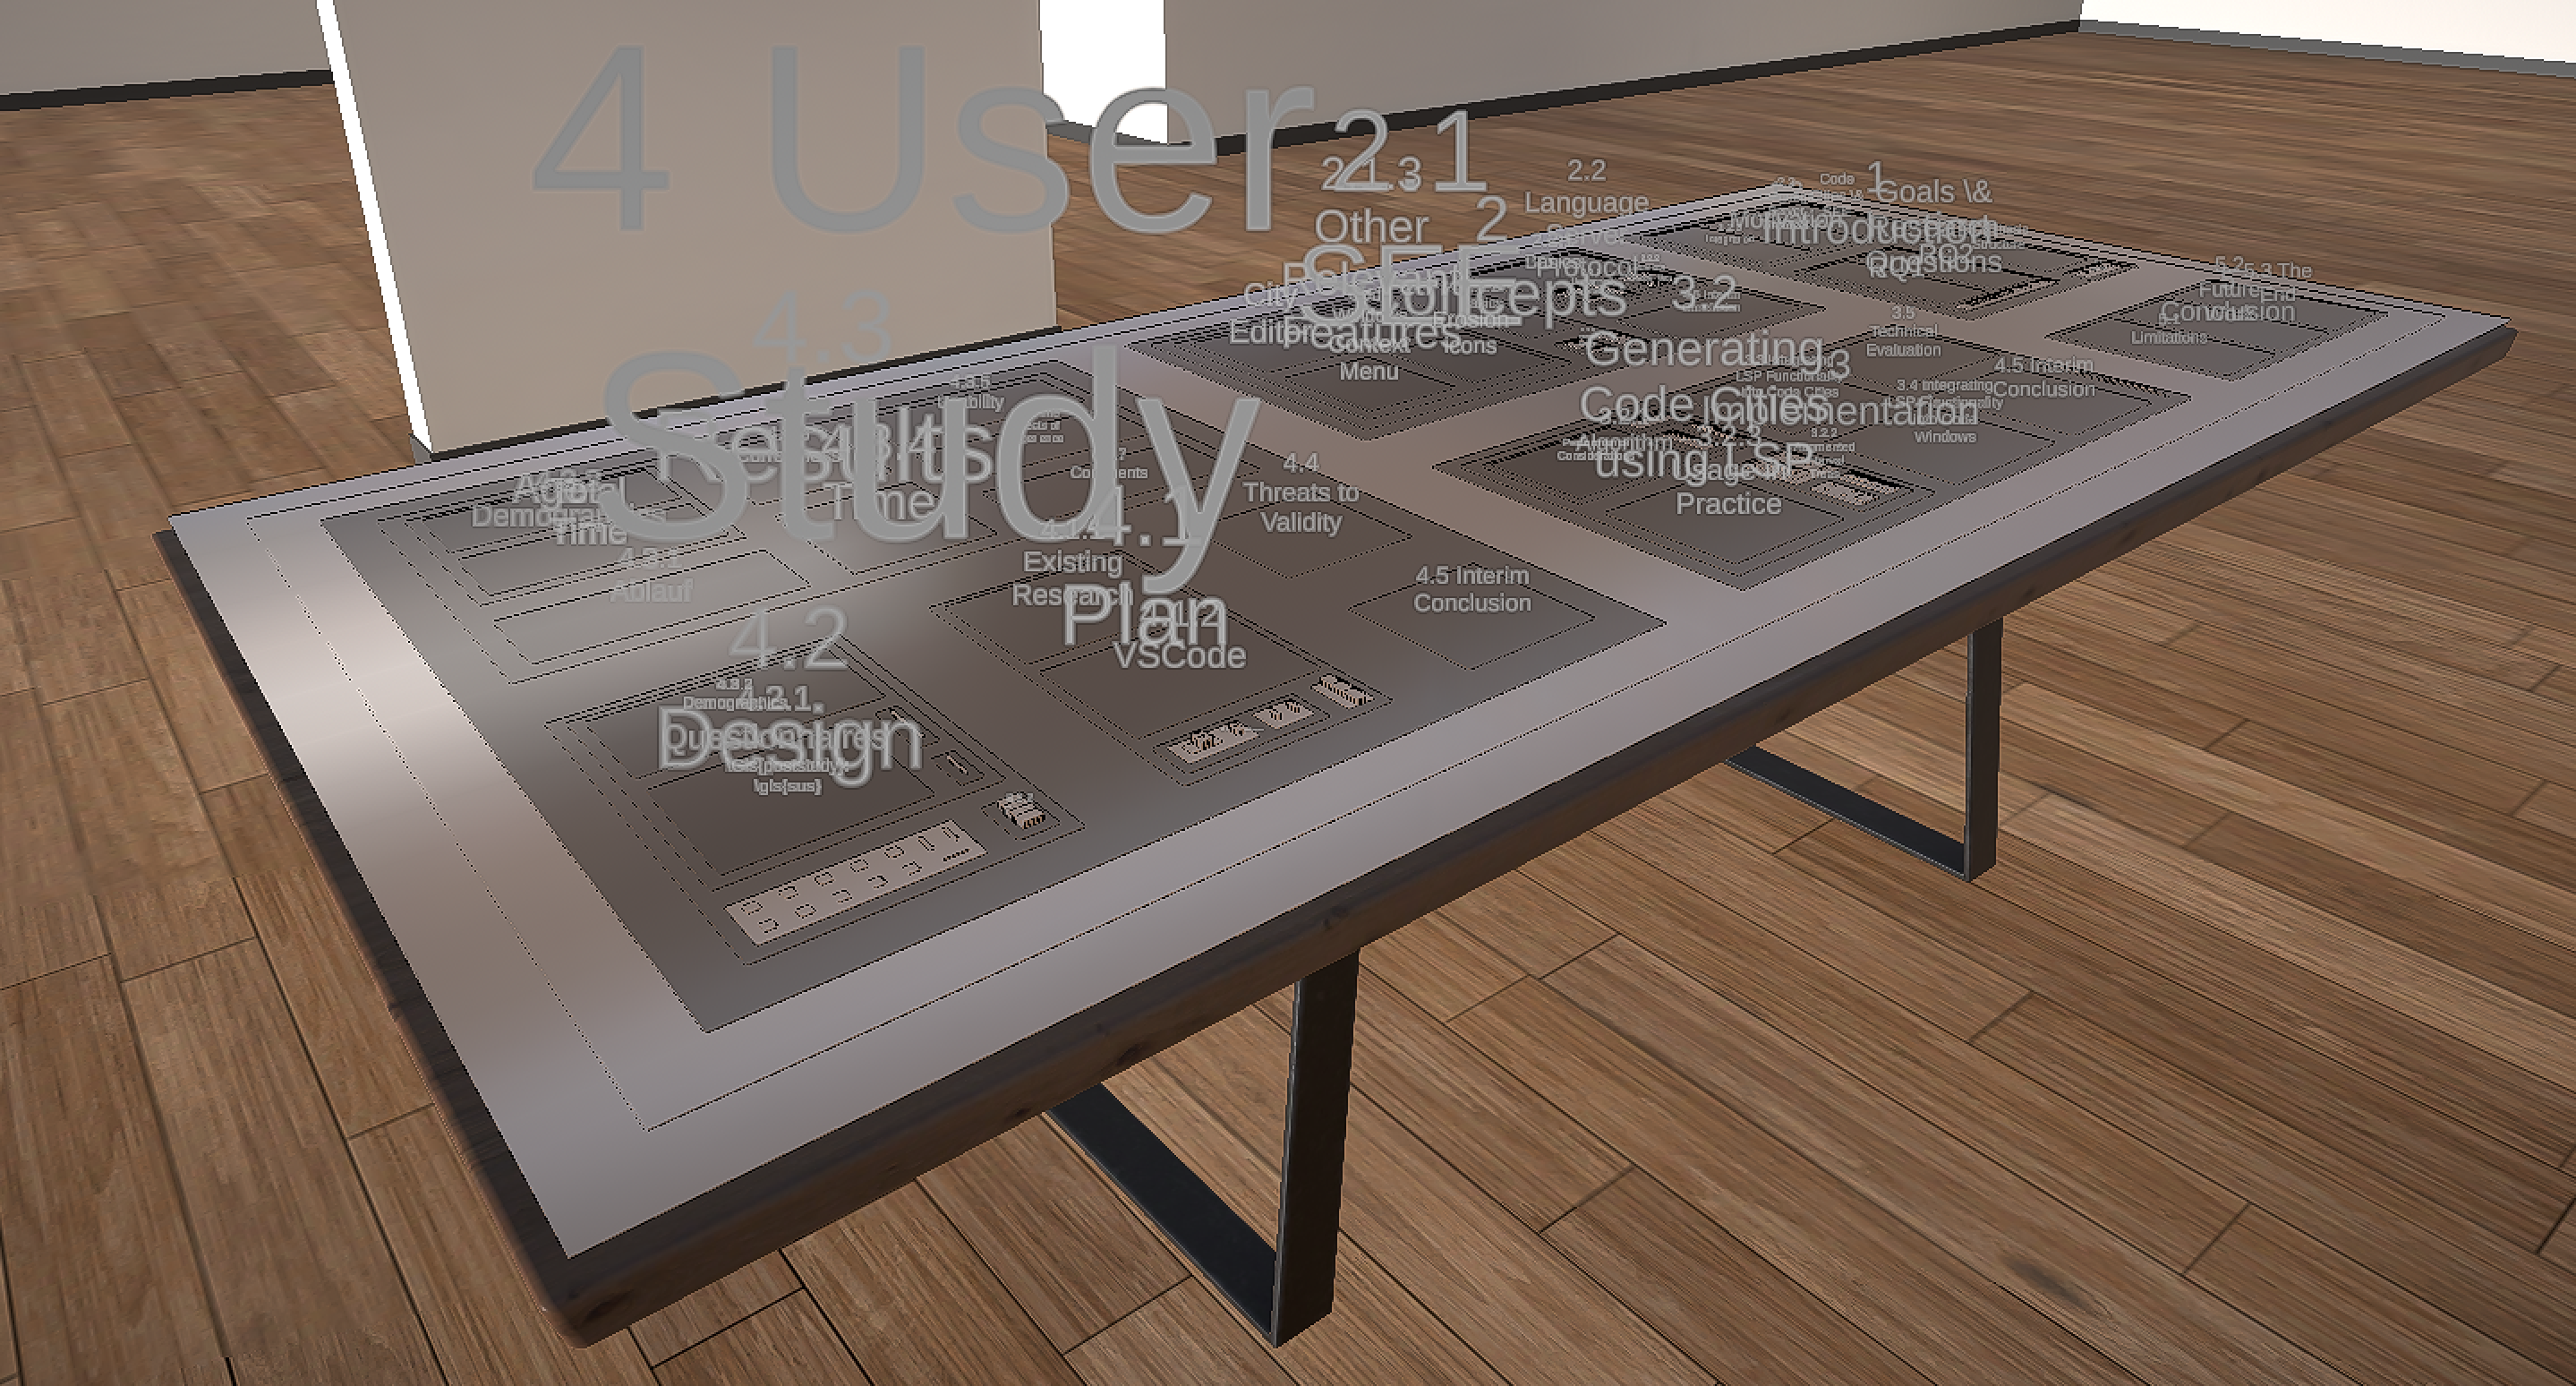
\includegraphics[width=\textwidth]{MasterCity}
		\caption{\Gls{city} for this master's thesis.}\label{fig:mastercity}
	\end{subfigure}
	\begin{subfigure}{0.5\textwidth}
		\centering
		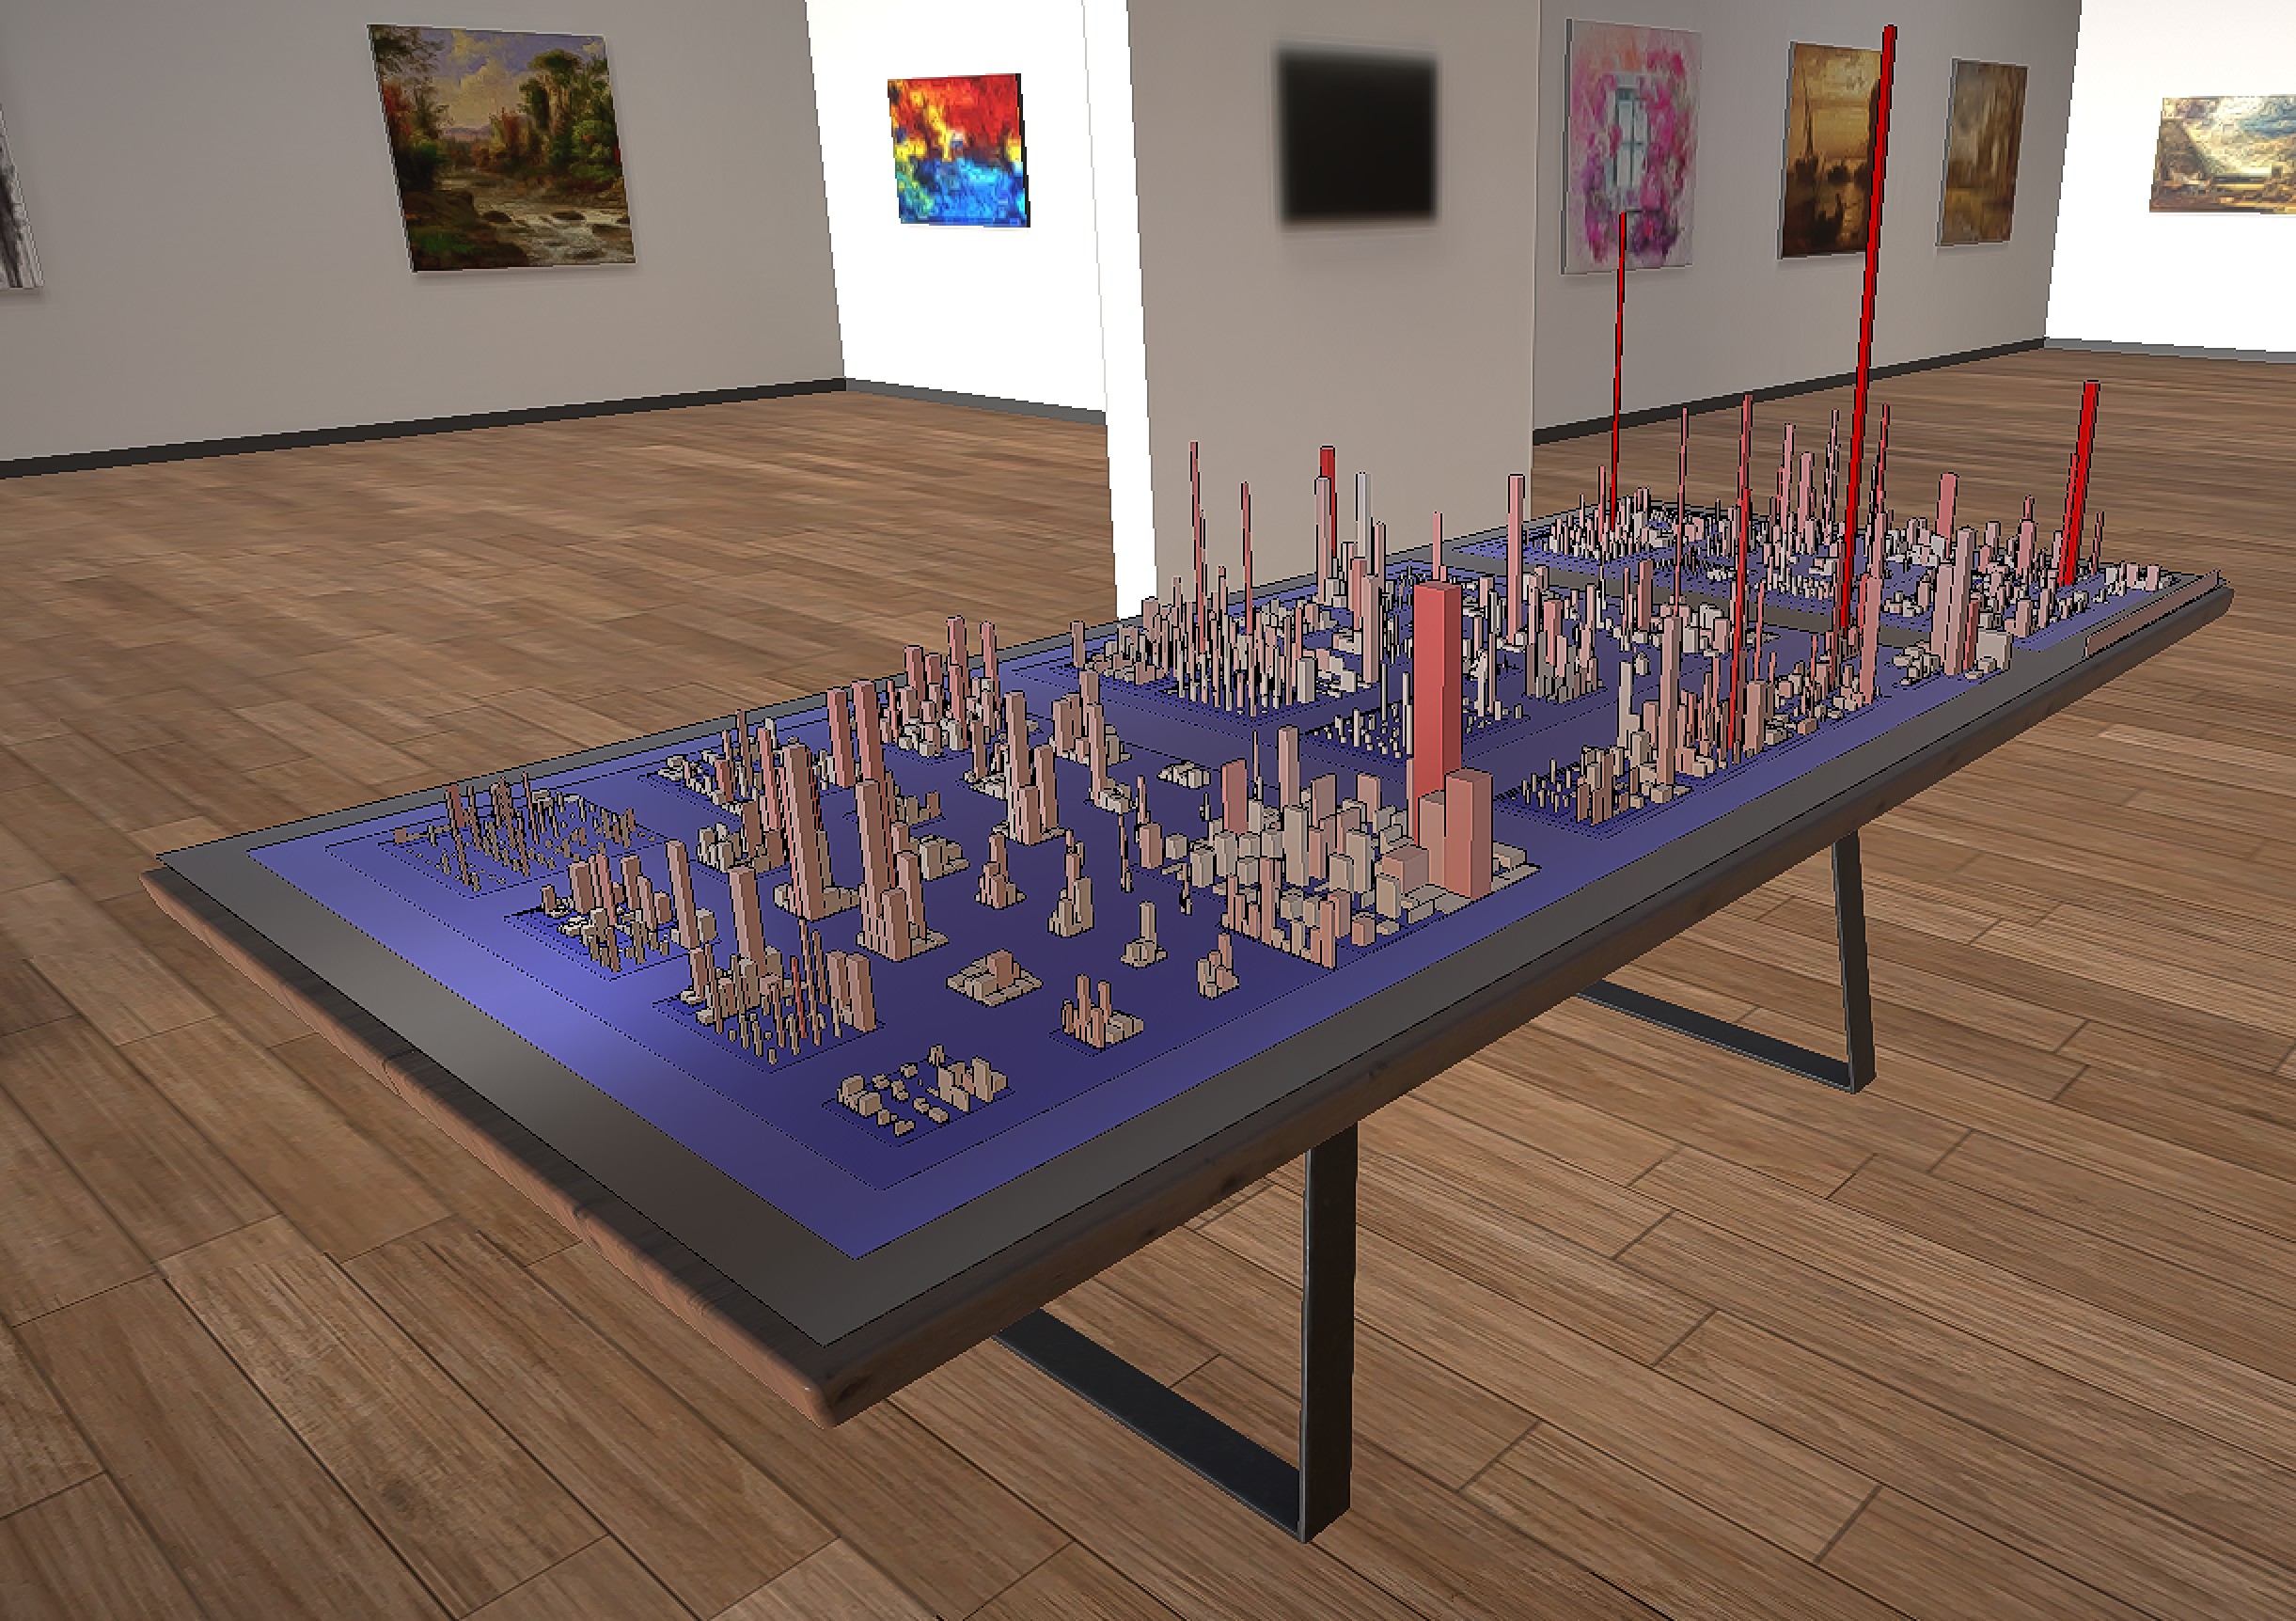
\includegraphics[width=\textwidth]{JabCity}
		\caption{\Gls{city} for the JabRef project.}\label{fig:jabcity}
	\end{subfigure}
	\begin{subfigure}{0.5\textwidth}
		\centering
		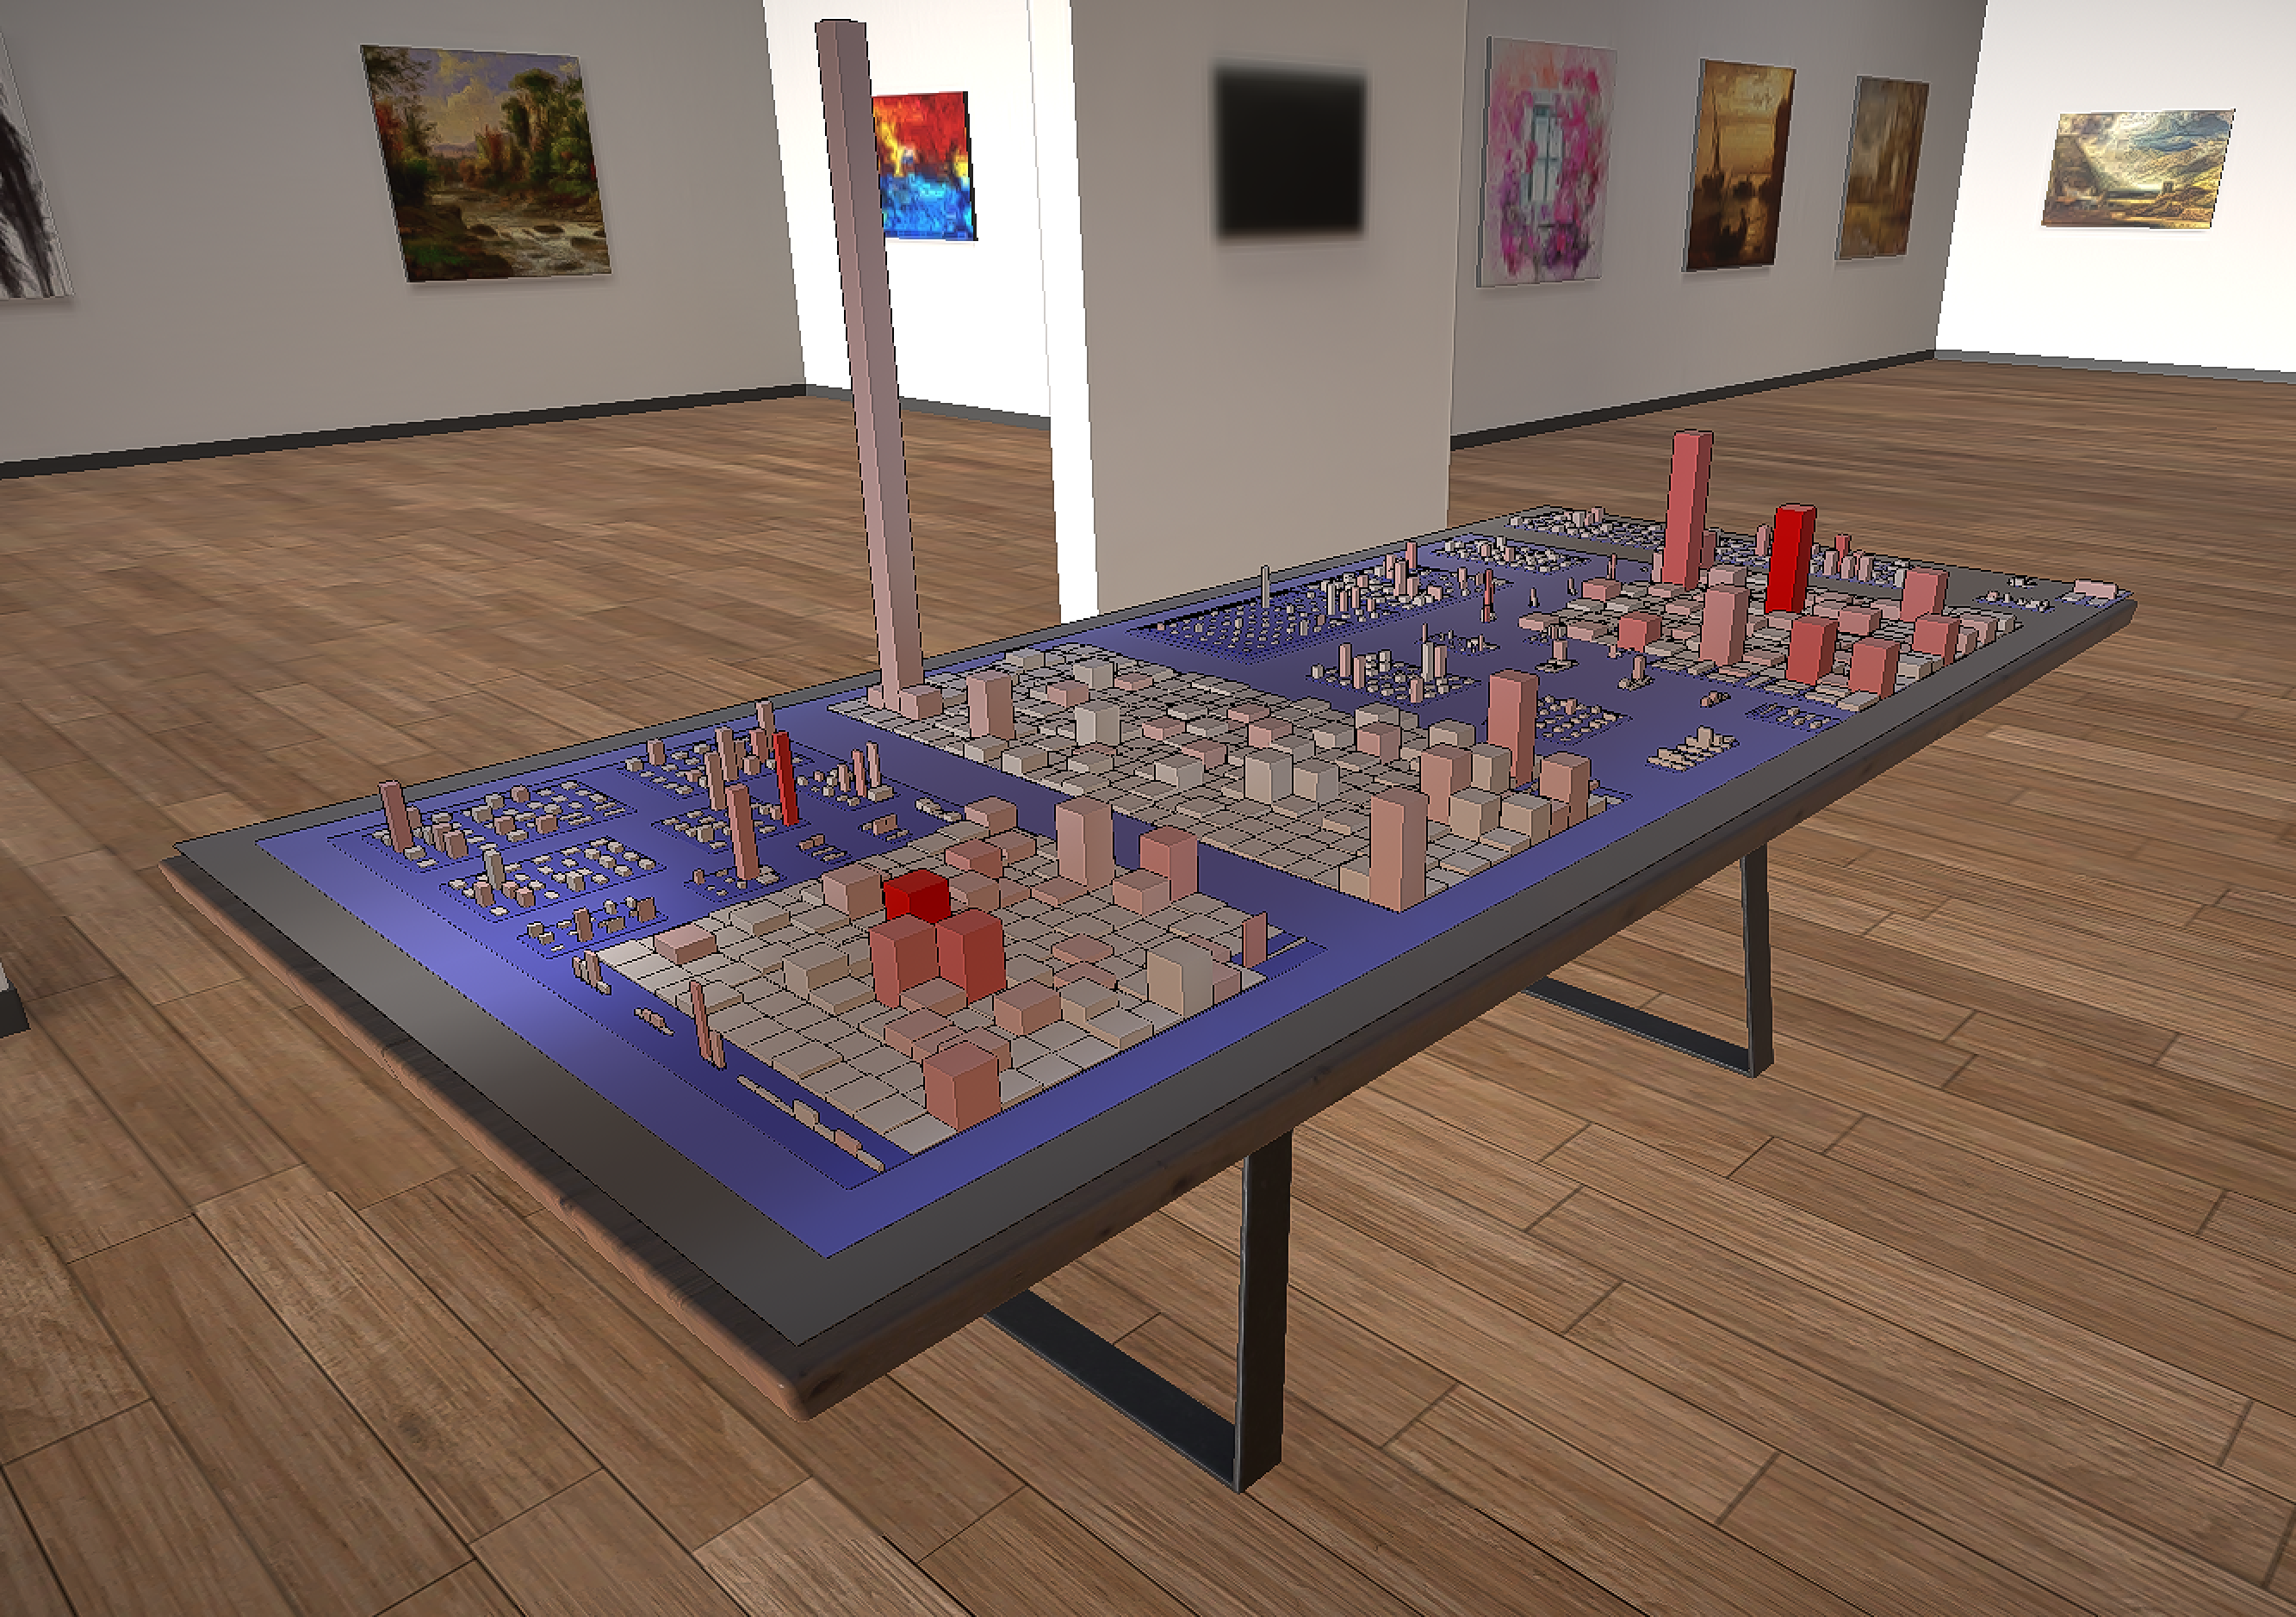
\includegraphics[width=\textwidth]{SpotCity}
		\caption{\Gls{city} for the SpotBugs project.}\label{fig:spotcity}
	\end{subfigure}
	\caption{Sample \glspl{city} generated using the \gls{lsp} algorithm introduced in this chapter.}\label{fig:gencities}
\end{figure}

Finally, we can take a look at the generated \glspl{city} shown in \cref{fig:gencities}.
No edges are shown in those diagrams---they would clutter up the images too much due to their high number.
While I am not as familiar with the source code of JabRef and SpotBugs, the ones for the first four projects seem correct to me on first glance:
\Cref{fig:bachcity,fig:mastercity} show the sections of both theses, and the biggest components correspond to the largest parts in the theses themselves (\eg, the evaluation section from my bachelor thesis was by far the longest part of it, which is reflected in that building being the largest in the \gls{city}).
We can even see some diagnostics for the bachelor's thesis, probably about unused labels.
The two Rust projects in \cref{fig:aaocity,fig:dcafcity} also match up with my knowledge of them, such as the biggest function being what I thought it would be.

There is one weird aspect here, though, that is not present in other languages, namely that there seem to be duplicated empty modules.
For example, in \cref{fig:aaocity}, we can see an empty grey \proptt{re} component, even though the regular expressions contained in the corresponding module are shown elsewhere in the city.
My guess is that there is a mismatch between Rust modules and files that is not handled correctly either by the Rust Analyzer or by my algorithm.
Still, this should not be a big problem, as the structure of the \gls{city} still reflects the original project apart from those empty modules.

\section{Interim Conclusion}\label{sec:implconclusion}
In this chapter, we covered how we implemented the various aspects of the \gls{lsp} integration, placing a special focus on the generation algorithm for \glspl{city}.
We closed out the chapter by evaluating the implementation and benchmarking its performance.

The technical evaluation revealed that the implementation does work well for the tested projects and that the implemented optimizations make sense, but the total runtime still is not really at the level where this system can be used productively for larger projects.
For example, generating a city for SpotBugs, a project with around \qty{200000}{\loc}, took almost ten minutes---and this was with almost all node and edge types being disabled!
Actually generating a \gls{city} for projects on the order of \qty{1000000}{\loc} from \gls{lsp} information with all available information being present (\ie, all nodes, all edges, all diagnostics) still seems intractable, but I am unsure whether this is due to additional inefficiencies in the algorithm or if the \glspl{ls} themselves are at fault.\footnote{
	Of course, this is a slightly unfair assessment---\glspl{ls} were never developed with the intent to be used in high-throughput scenarios like this, only for moderate use in \glspl{ide}.
}
Thus, we have to answer our first research question \textsf{RQ1} with caveats:
While it is feasible to generate \glspl{city} using the \glsentrylong{lsp}, more research and work needs to be done for this to work well with very large software projects.

\Cref{tab:code} contains a summary of all pull requests created for this thesis, along with the number of added and deleted lines.
There is one more pull request here that I have not mentioned yet, since it only contains disparate fixes and small additions that were done for the user study that we will talk about in the next chapter.
The fixes for this pull request were a mix of things I noticed myself while designing the user study and bugs noticed while conducting the pilot study (see \cref{subsec:procedure}).
There are two relevant features here that we should quickly go over:
\begin{itemize}
	\item Edges of a certain type can be hidden, causing them to only be shown when hovering over nodes they are connected to.
	      This mitigates the problem of too many edges obscuring and cluttering the \gls{city}.
	\item \emph{Transitive edge animations:}
	      When an edge is revealed by hovering above it, the "next" connected edge is repeatedly revealed as well.
	      For example, when this is enabled for "extend" edges, hovering over a class node will gradually reveal the path to the \gls{base}.
	      I recommend watching the explanatory video for the user study to get an intuitive understanding about this\footnote{
		      See \web{https://www.youtube.com/watch?v=WE21naXp\_YM}{2024-12-28}.
	      }.
\end{itemize}

\begin{table*}[htbp]
	\newcommand{\githubpr}[2]{\href{https://github.com/#1/pull/#2}{\proptt{#1\##2}}}
	\newcommand{\diffsum}[2]{\textcolor{Green}{\ensuremath{#1}} & \textcolor{Red}{\ensuremath{#2}}}
	\caption{All submitted pull requests done as part of this thesis.}\label{tab:code}
	\begin{tabular}{@{}llrl@{}}
		\toprule
		\multicolumn{1}{c}{\multirow{2}{*}{\textbf{Summary}}} & \multicolumn{1}{c}{\multirow{2}{*}{\textbf{Pull Request URI}}} & \multicolumn{2}{c}{\>\> $\mathbf{\Delta}$ \textbf{LOC}}                \\
		                                                      &                                                                & $\mathbf{+}$                                            & $\mathbf{-}$ \\
		\midrule
		Cleanup of \gls{lsp} specification                    & \githubpr{microsoft/language-server-protocol}{1886}            & \diffsum{475}{453}                                                     \\
		Preparing \SEE{} for \gls{lsp} integration            & \githubpr{uni-bremen-agst/SEE}{687}                            & \diffsum{282}{2773}                                                    \\
		Introducing \tt{Source.\Gls{range}}                   & \githubpr{uni-bremen-agst/SEE}{715}                            & \diffsum{392}{313}                                                     \\
		Generating \glspl{city} using \gls{lsp}               & \githubpr{uni-bremen-agst/SEE}{727}                            & \diffsum{3475}{180}                                                    \\
		\gls{lsp} functions in \glspl{city}                   & \githubpr{uni-bremen-agst/SEE}{747}                            & \diffsum{1139}{432}                                                    \\
		\gls{lsp} functions in \glspl{window}                 & \githubpr{uni-bremen-agst/SEE}{751}                            & \diffsum{4080}{2024}                                                   \\
		Preparing \SEE{} for user study                       & \githubpr{uni-bremen-agst/SEE}{772}                            & \diffsum{541}{150}                                                     \\
		\bottomrule
	\end{tabular}
	\caption*{\footnotesize Only C\# line changes have been counted in \SEE{} pull requests.\\
		GitHub pull requests are specified in the format \tt{namespace/repository\#PR\_number}.
	}

\end{table*}

\chapterendornament{77}{0.2}
